\documentclass[a4paper,12pt,twoside]{memoir}

% Castellano
\usepackage[spanish,es-tabla]{babel}
\selectlanguage{spanish}
\usepackage[utf8]{inputenc}
\usepackage[T1]{fontenc}
\usepackage{lmodern} % scalable font
\usepackage{microtype}
\usepackage{placeins}
\usepackage{eurosym}

\usepackage{longtable,booktabs}
\RequirePackage{booktabs}
\RequirePackage[table]{xcolor}
\RequirePackage{xtab}
\RequirePackage{multirow}

% Formato para referenciar nombre de comandos, bibliotecas, archivo 
\newcommand{\code}[1]{\texttt{#1}}

% Palabras en Inglés
\newcommand{\english}[1]{\emph{#1}}

% Bibliography management
\usepackage[numbers,sort]{natbib}


% Links
\usepackage[colorlinks]{hyperref}
\hypersetup{
  colorlinks,
  linkcolor={green!40!black},
  citecolor={blue!50!black},
  urlcolor={blue!80!black}
}

% Ecuaciones
\usepackage{amsmath}

% Rutas de fichero / paquete
\newcommand{\ruta}[1]{{\sffamily #1}}

% Párrafos
\nonzeroparskip


% Imagenes
\usepackage{graphicx}
\newcommand{\imagen}[2]{
	\begin{figure}[!h]
		\centering
		\includegraphics[width=0.9\textwidth]{#1}
		\caption{#2}\label{fig:#1}
	\end{figure}
	\FloatBarrier
}

\newcommand{\imagenflotante}[2]{
	\begin{figure}%[!h]
		\centering
		\includegraphics[width=0.9\textwidth]{#1}
		\caption{#2}\label{fig:#1}
	\end{figure}
}



% El comando \figura nos permite insertar figuras comodamente, y utilizando
% siempre el mismo formato. Los parametros son:
% 1 -> Porcentaje del ancho de página que ocupará la figura (de 0 a 1)
% 2 --> Fichero de la imagen
% 3 --> Texto a pie de imagen
% 4 --> Etiqueta (label) para referencias
% 5 --> Opciones que queramos pasarle al \includegraphics
% 6 --> Opciones de posicionamiento a pasarle a \begin{figure}
\newcommand{\figuraConPosicion}[6]{%
  \setlength{\anchoFloat}{#1\textwidth}%
  \addtolength{\anchoFloat}{-4\fboxsep}%
  \setlength{\anchoFigura}{\anchoFloat}%
  \begin{figure}[#6]
    \begin{center}%
      \Ovalbox{%
        \begin{minipage}{\anchoFloat}%
          \begin{center}%
            \includegraphics[width=\anchoFigura,#5]{#2}%
            \caption{#3}%
            \label{#4}%
          \end{center}%
        \end{minipage}
      }%
    \end{center}%
  \end{figure}%
}

%
% Comando para incluir imágenes en formato apaisado (sin marco).
\newcommand{\figuraApaisadaSinMarco}[5]{%
  \begin{figure}%
    \begin{center}%
    \includegraphics[angle=90,height=#1\textheight,#5]{#2}%
    \caption{#3}%
    \label{#4}%
    \end{center}%
  \end{figure}%
}
% Para las tablas
\newcommand{\otoprule}{\midrule [\heavyrulewidth]}
%
% Nuevo comando para tablas pequeñas (menos de una página).
\newcommand{\tablaSmall}[5]{%
 \begin{table}
  \begin{center}
   \rowcolors {2}{gray!35}{}
   \begin{tabular}{#2}
    \toprule
    #4
    \otoprule
    #5
    \bottomrule
   \end{tabular}
   \caption{#1}
   \label{tabla:#3}
  \end{center}
 \end{table}
}

%
%Para el float H de tablaSmallSinColores
\usepackage{float}

%
% Nuevo comando para tablas pequeñas (menos de una página).
\newcommand{\tablaSmallSinColores}[5]{%
 \begin{table}[H]
  \begin{center}
   \begin{tabular}{#2}
    \toprule
    #4
    \otoprule
    #5
    \bottomrule
   \end{tabular}
   \caption{#1}
   \label{tabla:#3}
  \end{center}
 \end{table}
}

\newcommand{\tablaApaisadaSmall}[5]{%
\begin{landscape}
  \begin{table}
   \begin{center}
    \rowcolors {2}{gray!35}{}
    \begin{tabular}{#2}
     \toprule
     #4
     \otoprule
     #5
     \bottomrule
    \end{tabular}
    \caption{#1}
    \label{tabla:#3}
   \end{center}
  \end{table}
\end{landscape}
}

%
% Nuevo comando para tablas grandes con cabecera y filas alternas coloreadas en gris.
\newcommand{\tabla}[6]{%
  \begin{center}
    \tablefirsthead{
      \toprule
      #5
      \otoprule
    }
    \tablehead{
      \multicolumn{#3}{l}{\small\sl continúa desde la página anterior}\\
      \toprule
      #5
      \otoprule
    }
    \tabletail{
      \hline
      \multicolumn{#3}{r}{\small\sl continúa en la página siguiente}\\
    }
    \tablelasttail{
      \hline
    }
    \bottomcaption{#1}
    \rowcolors {2}{gray!35}{}
    \begin{xtabular}{#2}
      #6
      \bottomrule
    \end{xtabular}
    \label{tabla:#4}
  \end{center}
}

%
% Nuevo comando para tablas grandes con cabecera.
\newcommand{\tablaSinColores}[6]{%
  \begin{center}
    \tablefirsthead{
      \toprule
      #5
      \otoprule
    }
    \tablehead{
      \multicolumn{#3}{l}{\small\sl continúa desde la página anterior}\\
      \toprule
      #5
      \otoprule
    }
    \tabletail{
      \hline
      \multicolumn{#3}{r}{\small\sl continúa en la página siguiente}\\
    }
    \tablelasttail{
      \hline
    }
    \bottomcaption{#1}
    \begin{xtabular}{#2}
      #6
      \bottomrule
    \end{xtabular}
    \label{tabla:#4}
  \end{center}
}

%
% Nuevo comando para tablas grandes sin cabecera.
\newcommand{\tablaSinCabecera}[5]{%
  \begin{center}
    \tablefirsthead{
      \toprule
    }
    \tablehead{
      \multicolumn{#3}{l}{\small\sl continúa desde la página anterior}\\
      \hline
    }
    \tabletail{
      \hline
      \multicolumn{#3}{r}{\small\sl continúa en la página siguiente}\\
    }
    \tablelasttail{
      \hline
    }
    \bottomcaption{#1}
  \begin{xtabular}{#2}
    #5
   \bottomrule
  \end{xtabular}
  \label{tabla:#4}
  \end{center}
}



\definecolor{cgoLight}{HTML}{EEEEEE}
\definecolor{cgoExtralight}{HTML}{FFFFFF}

%
% Nuevo comando para tablas grandes sin cabecera.
\newcommand{\tablaSinCabeceraConBandas}[5]{%
  \begin{center}
    \tablefirsthead{
      \toprule
    }
    \tablehead{
      \multicolumn{#3}{l}{\small\sl continúa desde la página anterior}\\
      \hline
    }
    \tabletail{
      \hline
      \multicolumn{#3}{r}{\small\sl continúa en la página siguiente}\\
    }
    \tablelasttail{
      \hline
    }
    \bottomcaption{#1}
    \rowcolors[]{1}{cgoExtralight}{cgoLight}

  \begin{xtabular}{#2}
    #5
   \bottomrule
  \end{xtabular}
  \label{tabla:#4}
  \end{center}
}




\graphicspath{ {./img/} }

% Capítulos
\chapterstyle{bianchi}
\newcommand{\capitulo}[2]{
	\setcounter{chapter}{#1}
	\setcounter{section}{0}
	\chapter*{#2}
	\addcontentsline{toc}{chapter}{#2}
	\markboth{#2}{#2}
}

% Apéndices
\renewcommand{\appendixname}{Apéndice}
\renewcommand*\cftappendixname{\appendixname}

\newcommand{\apendice}[1]{
	%\renewcommand{\thechapter}{A}
	\chapter{#1}
}

\renewcommand*\cftappendixname{\appendixname\ }

% Formato de portada
\makeatletter
\usepackage{xcolor}
\newcommand{\tutor}[1]{\def\@tutor{#1}}
\newcommand{\course}[1]{\def\@course{#1}}
\definecolor{cpardoBox}{HTML}{E6E6FF}
\def\maketitle{
  \null
  \thispagestyle{empty}
  % Cabecera ----------------
\noindent
\includegraphics[width=\textwidth]{cabecera}\vspace{1cm}%
  \vfill
  % Título proyecto y escudo informática ----------------
  \colorbox{cpardoBox}{%
    \begin{minipage}{.8\textwidth}
      \vspace{.5cm}\Large
      \begin{center}
      \textbf{TFG del Grado en Ingeniería Informática}\vspace{.6cm}\\
      \textbf{\LARGE\@title{}}
      \end{center}
      \vspace{.2cm}
    \end{minipage}

  }%
  \hfill\begin{minipage}{.20\textwidth}
    
\includegraphics[width=\textwidth]{escudoInfor}
  \end{minipage}
  \vfill
  % Datos de alumno, curso y tutores ------------------
  \begin{center}%
  {%
    \noindent\LARGE
    Presentado por\\ \@author{}\\ 
    en Universidad de Burgos --- \@date{}\\
    Tutores: \@tutor{}\\
  }%
  \end{center}%
  \null
  \cleardoublepage
  }
\makeatother
\newcommand{\nombre}{José Eduardo Risco Sánchez-Cortés} %%% cambio de comando

% Datos de portada
\title{{\Huge SurveyingPointCode}\\[0.5cm]Automatización del proceso de delineación a partir de datos de un Levantamiento Topográfico.}
\author{\nombre}
\tutor{Dr. César García-Osorio\\ y Dr. Carlos López Nozal}
\date{\today}

\begin{document}

\maketitle



\cleardoublepage



%%%%%%%%%%%%%%%%%%%%%%%%%%%%%%%%%%%%%%%%%%%%%%%%%%%%%%%%%%%%%%%%%%%%%%%%%%%%%%%%%%%%%%%%



\frontmatter


\clearpage

% Indices
\tableofcontents

\clearpage

\listoffigures

\clearpage

\listoftables

\clearpage

\mainmatter

\appendix

\apendice{Plan de Proyecto Software}

\section{Introducción}

En este apartado se va a detallar como se ha llevado a cabo la planificación del proyecto. En la planificación es donde se estudia el coste tanto en tiempo, como en recursos y también, aunque sea un proyecto educacional, el coste económico y sus posibles beneficios.

Con los resultados obtenidos realizaremos la planificación temporal del proyecto y el estudio de viabilidad del mismo. 

\section{Planificación temporal}

Como ya se ha mencionado en el inicio del proyecto, se ha optado por seguir la metodología ágil \emph{Scrum}. Se ha intentado seguirla fielmente, con la salvedad de que normalmente en este tipo de proyectos participan varias personas y en este ha participado solo una persona, con la supervisión del tutor.

\begin{figure}[H]
	\centering
	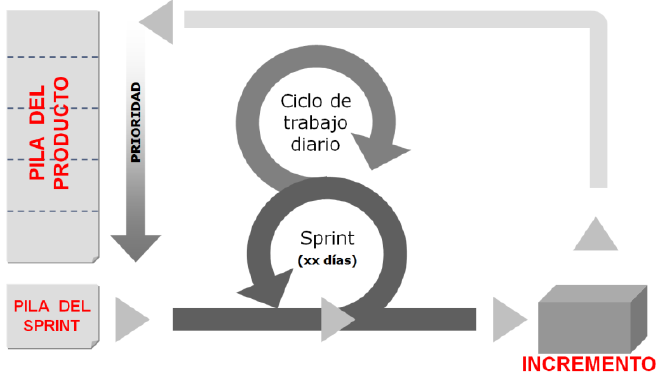
\includegraphics[width=0.6\textwidth]{Scrum}
	\caption{Diagrama del ciclo iterativo \emph{Scrum}.}
	\label{fig:Scrum}
\end{figure}

\emph{Scrum} se basa en aplicar una estrategia de desarrollo incremental, que intenta mantener un ritmo de avance constante. Se planifican una serie de \emph{sprints} donde se debían desarrollar una serie de tareas completamente funcionales. La duración de estos \emph{sprints} era de una semana y al final de cada \emph{sprint} se realizaban reuniones para comprobar si se habían cumplido los objetivos y planificar el siguiente \emph{sprint}.

Los requisitos del sistema se registraron en dos formatos:

\begin{itemize}
\item \textbf{Pila del producto:} como una  lista ordenada de todo aquello que el propietario de producto cree que necesita el producto. La pila del producto nunca se da por completada; está en continuo crecimiento y evolución.

\item \textbf{Pila del \emph{sprint}:} como una lista de las tareas necesarias para construir las historias de usuario que se van a realizar en un \emph{sprint}. Refleja los requisitos vistos desde el punto de vista del equipo de desarrollo.
 
\end{itemize}

Para la gestión del proyecto se utilizó \emph{ZenHub}, en ella podíamos hacer el seguimiento de lo que está en revisión, lo que debe probarse, lo que se está haciendo o lo ya cerrado.


\begin{figure}[H]
	\centering
	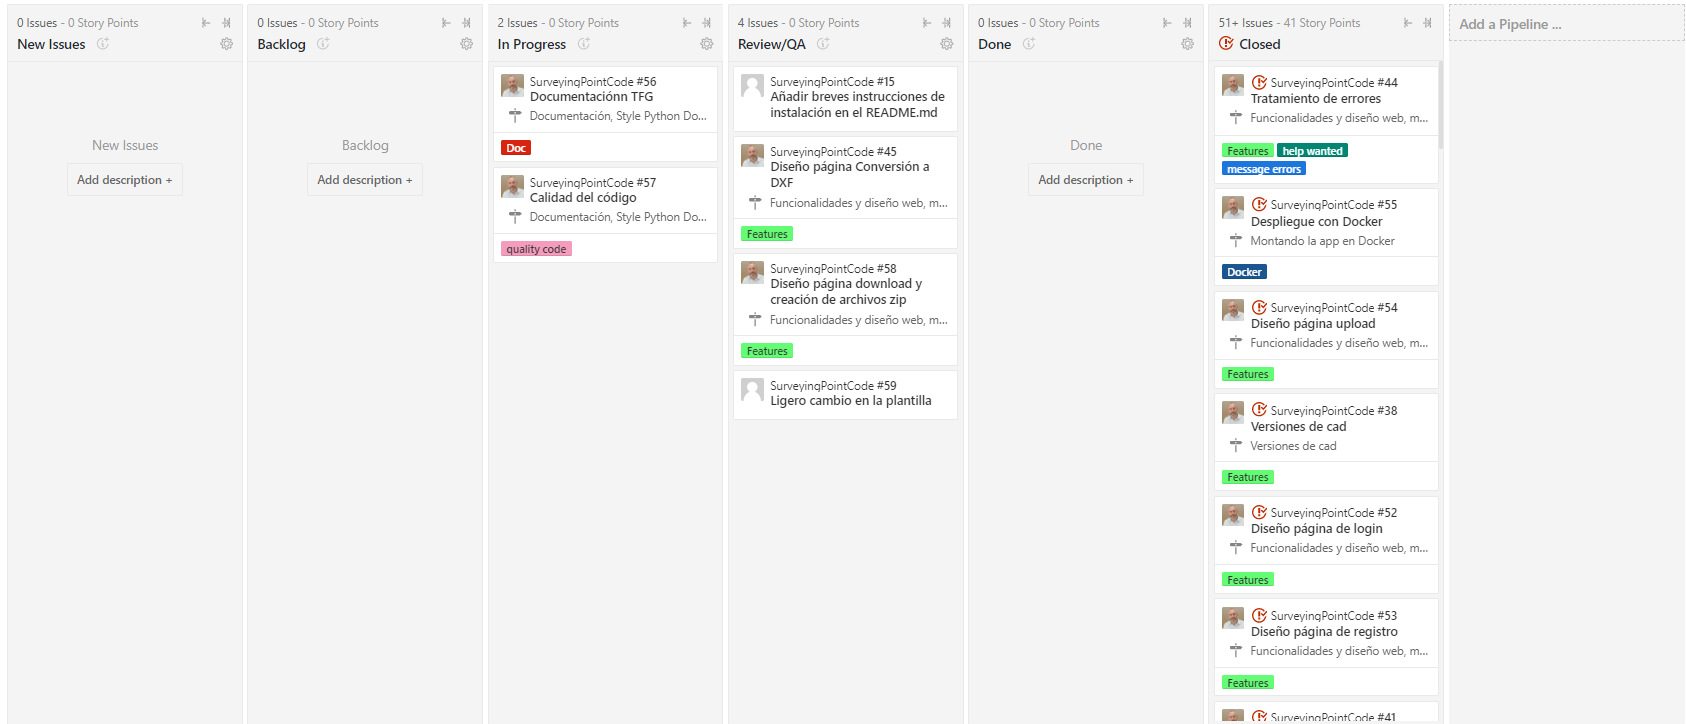
\includegraphics[width=0.9\textwidth]{ZenHub}
	\caption{Gestión de tareas con \emph{ZenHub} en una fase del proyecto.}
	\label{fig:ZenHub}
\end{figure}

A continuación se describen los diferentes \emph{sprints} que se han realizado:

\subsection{\emph{Sprint} 1 (24/01/2019 - 30/01/2019)}

En este primer \emph{sprint} y como primera toma de contacto con el proyecto, los objetivos planteados fueron los siguientes:

\begin{itemize}
\item Preparación del entorno de trabajo. El proyecto se iba a desarrollar en Python, se instaló la version \emph{Python 3.7} y como entorno de  la aplicación \emph{PyCharm 2019.1.1 Comunity Edition}.

\item Repaso de conocimientos en \emph{GIT} y creación del repositorio en \emph{GitHub}. Se refrescaron los conocimientos en \emph{GIT}, en algunos tutoriales  online como  \textit{git - la guía sencilla} \cite{git} y \textit{Tutorial de Git. Manual básico con ejemplos} \cite{git_1}

\item Formación en \emph{PEPs}. Para conocer bien las guías de estilo y la convenciones de \emph{Python}, se consultaron las guías PEP 8 y PEP 257, mencionadas en la memoria.

\item Formación en \LaTeX. Se consulto como guía principal, el libro Edición de Textos Científicos \LaTeX{}~\cite{latex}. Y como herramientas para realizar la memoria se instalaron las aplicaciones:\emph{Texmaker 5.0.3} y \emph{MikTex 2.9}.

\item Diseño del logotipo de la aplicación.

\begin{figure}[H]
	\centering
	
\includegraphics[width=0.3\textwidth]{SPC}
	\caption{Logo de \emph{SurveyingPointCode}.}
	\label{fig:SPC}
\end{figure}
 
\end{itemize}


\subsection{\emph{Sprint} 2 (31/01/2019 - 06/02/2019)}

Los objetivos planteados fueron los siguientes:

\begin{itemize}
\item Formalización de la entrada de datos: Se procede a formalizar la gramática que debe tener el archivo de entrada y se determina que:
el archivo de entrada será un archivo de texto, compuesto por una o múltiples líneas. Estas líneas serán los puntos medidos en campo y cada línea tendrá la siguiente estructura:

número de punto, coordenada $x$, coordenada $y$, coordenada $z$, código
\begin{itemize}
\item El numero de punto debe ser de tipo \emph{integer}
\item Las coordenadas $x$, $y$, $z$ de tipo \emph{float} o \emph{integer}
\item El código de tipo string, pudiendo estar formado por letras, números y los signos '-' y '+'
\end{itemize}

\item Elección de una herramienta de análisis sintáctico: Se elige una herramienta de análisis sintáctico para poder validar los archivos de entrada. Las opciones eran:
\begin{itemize}
\item \emph{Ply}
\item \emph{ANTLR}
\item \emph{Flex Bison}
\end{itemize}
Nos decantamos por \emph{Ply} ya que está implementada completamente
en \emph{Python} y encaja perfectamente con la filosofía de realizar la mayor parte del proyecto con este lenguaje.

\item Creación de un prototipo: Se creó un prototipo que permitía indicarnos si el archivo de entrada era correcto o no. Se comprobó su funcionamiento con dos archivos, uno con la gramática correcta y otro gramática incorrecta, y el resultado fue satisfactorio en ambos casos. 

\end{itemize}


\subsection{\emph{Sprint} 3 (07/02/2019 - 13/02/2019)}

Como objetivo se planteó seguir con el desarrollo de este primer prototipo, ampliando sus funcionalidades. Se definieron las siguientes tareas:

\begin{itemize}
\item Organizar elementos en listas de capas: Se leerán las líneas del fichero de entrada (puntos medidos en campo) y se organizarán en una estructura de datos en forma de lista, donde cada lista contendrá los elementos (puntos) correspondientes a una misma capa. Se obtuvo un resultado correcto.

\item Identificar y organizar los diferentes tipos de líneas: Se pretende identificar todos los puntos que forman unas línea, y almacenar todas las líneas existentes en estructuras de datos. Se obtuvo un resultado correcto.

\item Comenzando con biblioteca \texttt{ezdxf}: Se comienza a estudiar la biblioteca \texttt{ezdxf} y a realizar pequeñas pruebas, incluyendo estas en el prototipo. Dibujar las líneas y \emph{splines} de un fichero de entrada.

El resultado fue correcto, lo podemos ver en la siguiente imagen.

\begin{figure}[H]
	\centering
	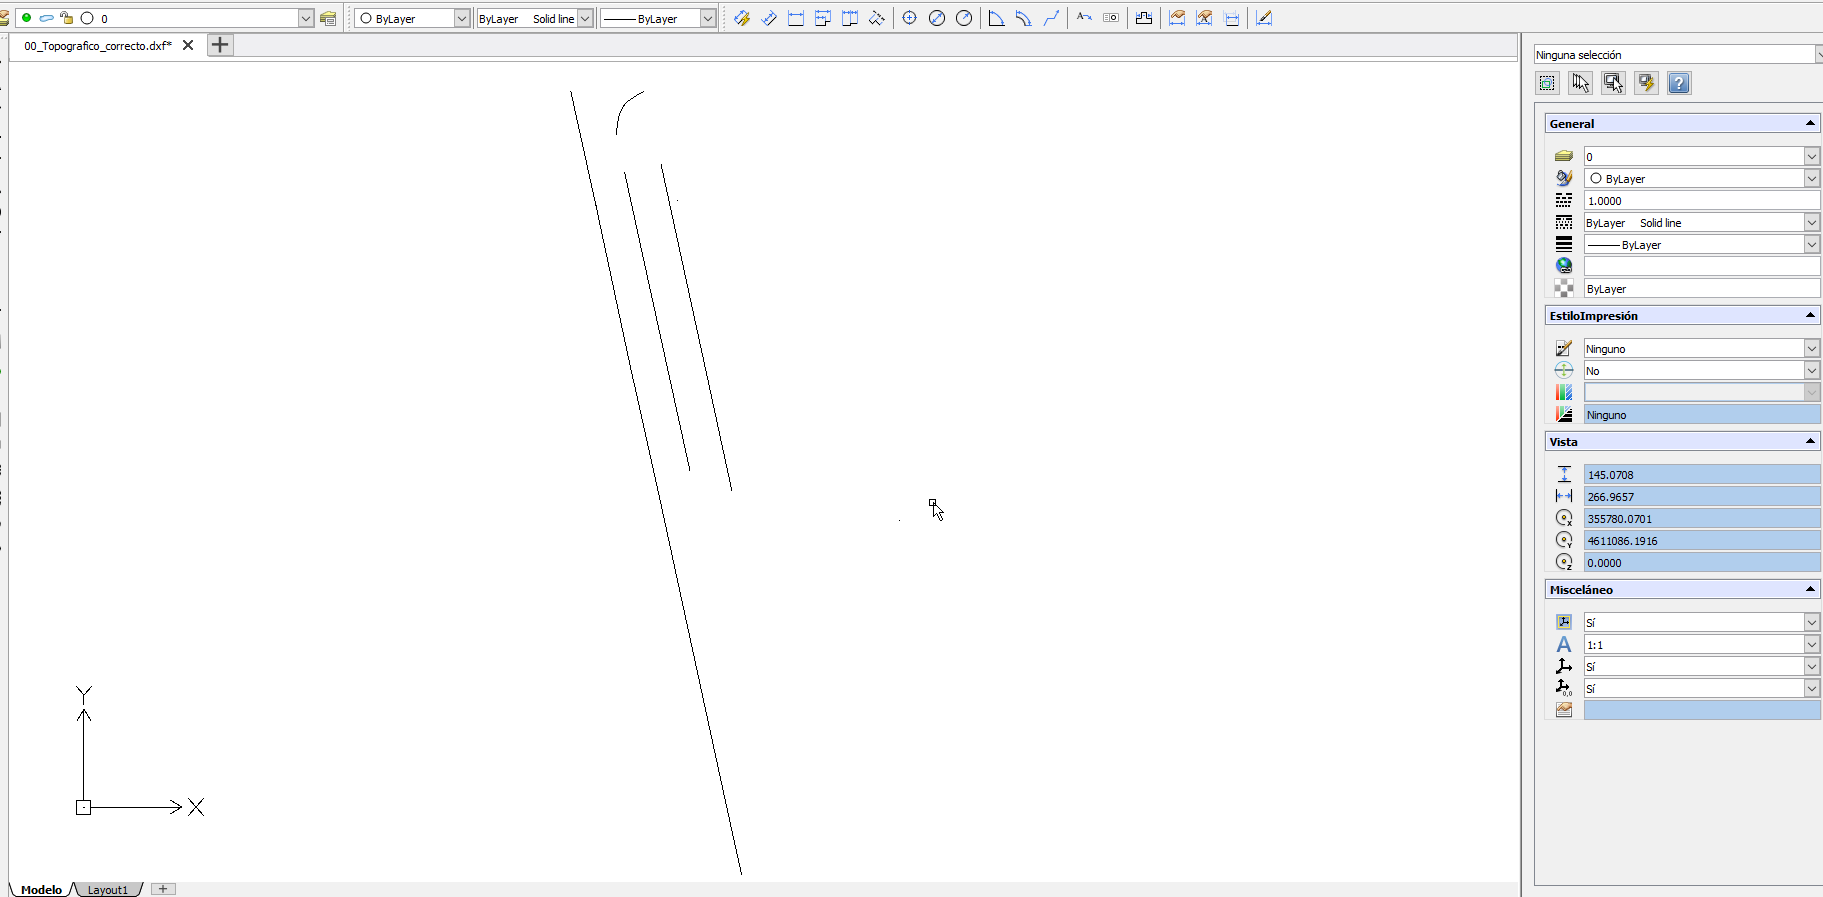
\includegraphics[width=0.6\textwidth]{proto_1}
	\caption{Logo de \emph{Dibujo con líneas y \emph{splines}.}}
	\label{fig:proto_1}
\end{figure}


\end{itemize}




\subsection{\emph{Sprint} 4 (14/02/2019 - 20/02/2019)}

Una vez acabado el primer prototipo funcional que podía validar un archivo, diferenciar las diferentes líneas y curvas, y generar un archivo DXF, el objetivo de este \emph{sprint} fue comenzar a crear un prototipo  basado en una aplicación Web, utilizando el \emph{micro framework} \texttt{Flask}. Para ello se definieron las siguientes tareas:

\begin{itemize}
\item Formación en \texttt{Flask}: Se consultó la documentación de \texttt{Flask} mencionada en la memoria.

\item Prototipo con \texttt{Flask}: Se creó un prototipo que permitía subir un archivo desde el equipo del usuario al servidor. Se obtuvo un resultado correcto.

\item Procesado del archivo subido y descarga del archivo DXF generado: El prototipo debería validar el archivo subido por el usuario, lo convertiría a DXF, y permitiría descargarlo en su equipo. Se obtuvo un resultado correcto.

\end{itemize}
 
Aquí empezó a trabajar con un entorno virtual creado en \emph{Anaconda}\footnote{\textsl{Anaconda}: \url{https://www.anaconda.com/}} por sugerencia del tutor.


\subsection{\emph{Sprint} 5 (21/02/2019 - 27/02/2019)}

Ya teníamos la aplicación Web funcionando, el siguiente paso sería la validación de usuarios, el uso de una base de datos y a ser posible comenzar a investigar con \emph{Docker} y alojar la base de datos en un contenedor. Para ello se definieron las siguientes tareas:

\begin{itemize}
\item Comenzando con \emph{Docker}: Se consultó la documentación de \\emph{Docker} mencionada en la memoria (ver apartado 5.3 Formación), y se configuró un contenedor \emph{PostGIS} para alojar la base de datos. También se configuró otro contenedor \emph{PgAdmin4} para poder administrar y ver las modificaciones en la base de datos más fácilmente. También serviría para probar como conectar dos contenedores entre sí.

\item Validación de usuarios: Se implementó la aplicación para que un usuario pudiera logearse y registrarse. Se diseño el modelo de la base datos y la base de datos se crearía automáticamente al arrancar la aplicación. Se utilizaron  las librerías \texttt{SQLAlchemy} y \texttt{Flask-Login}, mencionadas en la memoria, de las cuales se estudió su documentación. Se obtuvo un resultado correcto.
\end{itemize} 


\subsection{\emph{Sprint} 6 (08/03/2019 - 13/03/2019)}

Este \emph{sprint} se basó en el aprendizaje de \emph{HTML}, formularios y \emph{Bootstrap}. Incluyendo el tratamiento de mensajes \texttt{flash} en \texttt{Flask}.

También se estudió como incorporar un visor en el navegador, para poder visualizar el plano. Se estudiaron varias opciones:

\begin{itemize}
\item Convertir el archivo a formato SVG: Se convirtió el archivo DXF a SVG, con un conversor online\footnote{\textsl{convertio}: \url{https://convertio.co/es/dxf-svg/}}, pero el resultado obtenido no era lo esperado. Se probó con otros conversores siendo el resultado igual de malo, por lo que se descartó esta opción.
  
\item Usar el visor \emph{Three-Dxf}: \emph{Three-Dxf}\footnote{\textsl{Three-Dxf}: \url{https://github.com/gdsestimating/three-dxf}} en un visor en \emph{JavaScript}, para archivos DXF, que se podría incorporar a cualquier aplicación Web. En su documentación indicaba que soportaba los elementos que usábamos en nuestros DXF, como los tipos de líneas, tipos de símbolos, etc. Pero comprobándolo resultó que no era así, daba errores. Conseguía visualizar archivos muy simples, pero no los que necesitábamos en este proyecto.
\end{itemize}

Al final se descartó la idea de que la aplicación tuviera un visor incorporado.

\subsection{\emph{Sprint} 7 (14/03/2019 - 20/03/2019)}

Este \emph{sprint} se basó en implementar funciones que crearan los elementos del archivo DXF. Para ello se definieron las siguientes tareas:

\begin{itemize}
\item Creación de capas: Creación de capas en el DXF, a partir de los códigos del archivo de campo. Hay tres capas que se deberían crear siempre:
\begin{itemize}
	\item \emph{Point:} Capa que deberá contener todos los puntos.
 	\item \emph{Altitude:} Capa que deberá contener la altitud de todos los puntos. 	en forma de texto.
 	\item \emph{Label:}  Capa que deberá contener el código de todos los puntos, en 	forma de texto.
\end{itemize}
Se obtuvo un resultado correcto.

\item Inserción de puntos en el modelo: Se insertan todos los puntos del archivo de campo en el modelo del dibujo. Se dibujan también, los textos correspondientes al código y a la elevación del punto, cada uno en su correspondiente capa, todo ello interpretando la codificación. Se obtuvo un resultado correcto.

\item Creación de circunferencias: Se crearían círculos, a partir de un punto y un radio, y se guardaría en su correspondiente capa, todo ello interpretando la codificación. Se obtuvo un resultado correcto.  

\item Creación de líneas: Se crearían líneas, a partir de una serie de puntos, y se guardarían en su correspondiente capa, todo ello interpretando la codificación. Se obtuvo un resultado correcto. 

\item Creación de cuadrados: Se crearían cuadrados, a partir de dos puntos, y se guardarían en su correspondiente capa, todo ello interpretando la codificación. El cuadrado siempre se dibujaría a la derecha de la alíneación definida por estos dos puntos. Se obtuvo un resultado correcto.   

\item Creación de rectángulos: Se crearían rectángulos, a partir de tres puntos, y se guardarían en su correspondiente capa, todo ello interpretando la codificación. Se obtuvo un resultado correcto.   

\item Uso de puntos no medidos en campo: Se utilizarían puntos no medidos en campo para la generación de líneas y se guardarían en su correspondiente capa, todo ello interpretando la codificación. Se obtuvo un resultado correcto.
\end{itemize}

Una vez dibujados los elementos, se mejoró estéticamente el dibujo, modificando el tamaño de los textos y su posición respecto a los puntos.

\subsection{\emph{Sprint} 8 (21/03/2019 - 27/03/2019)}

En este \emph{sprint} se comenzó con la realización de test unitarios, estudiando las diferentes opciones. También como se podría  leer un archivo DXF proporcionado por el usuario, que contuviera símbolos en forma de bloques y una vez, incorporarlos al modelo de dibujo que queríamos generar. Para ello se definieron las siguientes tareas:

\begin{itemize}
\item Estudio de una biblioteca de Python para la realización de los test unitarios: Se consideraron las bibliotecas: \texttt{unittest}~\cite{unittest} y \texttt{pytest}~\cite{pytest}. La opción elegida fue \texttt{unittest}\, esta biblioteca ya se había usado durante la realización del grado.

\item Comienzo con los test unitarios.

\item Crear una función para cargar un archivo DXF.

\item Crear una función extraer los bloques del archivo DXF.

\item Incorporar los bloques al modelo del dibujo.

\item Asociar cada bloque con cada punto correspondiente, interpretando la codificación.

\end{itemize}

Se obtuvo un resultado correcto.
 
\subsection{\emph{Sprint} 8 (28/03/2019 - 03/04/2019)}

En este \emph{sprint} se comenzó a trabajar con la posibles versiones de CAD que podría generar la aplicación. También se comenzó a trabajar con el archivo de configuración de usuario, definiendo como sería su gramática e implementando un \emph{parser} para poder validarlo. Para ello se definieron las siguientes tareas:

\begin{itemize}
\item Versiones de CAD válidas: Se comprobaría la generación del archivo DXF en diferentes versiones y su validez. 

\item  Definición de gramática para el archivo de configuración de usuario.

\item Carga y validación del archivo de usuario.

\end{itemize}

En este \emph{sprint} se detecta un error en el uso de dos \emph{parsers} que se detalla en la memoria, \textit{Conflicto entre \emph{parsers}.}
 
\subsection{\emph{Sprint} 9 (04/04/2019 - 10/04/2019)}

En este \emph{sprint} se comenzó a trabajar con las sesiones de \texttt{Flask} multiusuario, se continuó con la definición, e implementación de funciones para la gestión del archivo de configuración de usuario y se soluciona el problema de del conflicto entre los dos \emph{parsers}. Para ello se definieron las siguientes tareas:

\begin{itemize}
\item Gestión del archivo de configuración de usuario. 

\item  Problema con el uso de dos \emph{parsers}.

\item Carga y validación del archivo de usuario.

\item Comienzo con las sesiones en \texttt{Flask}.
\end{itemize}

\subsection{\emph{Sprint} 10 (11/04/2019 - 24/04/2019)}

Este \emph{sprint} se consideró más largo, había una semana de vacaciones en medio. Básicamente se basó en completar las funcionalidades Web, el diseño de la Web, y el tratamiento de los mensajes de aviso. Para ello se definieron las siguientes tareas: 
 
\begin{itemize}
\item Añadir funcionalidades a la Web: Añadir o quitar botones, menús, etc.

\item  Mejorar el diseño de la Web: Página de inicio, barra de navegación superior, página de login, etc.

\item Tratamiento de errores: Ver e implementar las distintas formas, en que se presentaran los errores o mensajes de aviso al usuario.

\end{itemize}

Se solucionaron errores como, el surgido al añadir la letra <<ñ>> y la tildes, a la gramática del archivo de configuración (se puede ver la solución en la memoria \textit{ Codificación UTF-8}). También un error no detectado anteriormente en la función  \texttt{calculate\_azimut\_distance}, con un error de división por 0.
Además se comprobó que la paleta de colores de los programas CAD, no era la habitual (se puede ver la solución en la memoria \textit{ Paleta de colores en CAD})

\subsection{\emph{Sprint} 11 (25/04/2019 - 01/05/2019)}

En este \emph{sprint} y como parte final de la aplicación, el objetivo era facilitar su posterior despliegue en explotación mediante la utilización de contenedores \emph{Docker}. En un principio integrar la aplicación \texttt{Flask} y por último ejecutar todos los contenedores a la vez, con el uso de la herramienta \emph{Docker Compose}. Se obtuvo un resultado correcto.

\subsection{\emph{Sprint} 12 (02/05/2019 - 15/05/2019)}

En este \emph{sprint} se redacta la documentación del proyecto.

\subsection{\emph{Sprint} 13 (16/05/2019 - 22/05/2019)}

En este \emph{sprint} se continua con la redacción de la documentación del proyecto. Además se añaden las siguientes funcionalidades:

\begin{itemize}
\item Mensaje de \emph{Cookies}.

\item Tiempo de caducidad de la sesión de usuario

\item Mejora de la barra de navegación, incluyendo más funcionalidades.
\end{itemize}
Se consiguieron los objetivos.

\subsection{\emph{Sprint} 14 (23/05/2019 - 29/05/2019)}

En este \emph{sprint} se continuará con la redacción de la documentación del proyecto. Además se añadirán las siguientes funcionalidades:

\begin{itemize}
\item Ampliación de la base de datos para recoger estadísticas sobre el uso que hace de la aplicación cada usuario.

\item Mejora estética en la paleta de colores desplegable.

\item Revisión de las licencias.

\item Realización de un manual en vídeo.
\end{itemize}
Se consiguieron los objetivos.

\section{Estudio de viabilidad}

\subsection{Viabilidad económica}

En este apartado se analizan los costes del proyecto y también los posibles  beneficios del proyecto en caso de comercializarse.

\subsubsection{Costes}
\textbf{Costes de personal:}

El desarrollo del proyecto, tanto el tiempo empleado en la formación, como la implementación de la aplicación y redactar la documentación
generada, ha sido llevado a cabo por una sola persona durante 476 horas. Considerando 40 horas semanales, hemos trabajado 2.98  meses, por lo que redondeamos a 3 meses de trabajo a tiempo completo. Si consideramos que el trabajo lo ha realizado un programador junior, el salario será el siguiente:

\begin{longtable}[]{@{}lr@{}}
\toprule
\begin{minipage}[b]{0.38\columnwidth}\raggedright\strut
\textbf{Concepto}\strut
\end{minipage} & \begin{minipage}[b]{0.20\columnwidth}\raggedright\strut
\textbf{Coste}\strut
\end{minipage}\tabularnewline
\midrule
\endhead
\begin{minipage}[t]{0.38\columnwidth}\raggedright\strut
Salario mensual neto\strut
\end{minipage} & \begin{minipage}[t]{0.20\columnwidth}\raggedright\strut
1.088.29 \euro{}\strut
\end{minipage}\tabularnewline
\begin{minipage}[t]{0.38\columnwidth}\raggedright\strut
Retención IRPF (15\%)\strut
\end{minipage} & \begin{minipage}[t]{0.20\columnwidth}\raggedright\strut
296.,27 \euro{}\strut
\end{minipage}\tabularnewline
\begin{minipage}[t]{0.38\columnwidth}\raggedright\strut
Seguridad Social (29,9\%)\strut
\end{minipage} & \begin{minipage}[t]{0.20\columnwidth}\raggedright\strut
590,56 \euro{}\strut
\end{minipage}\tabularnewline
\begin{minipage}[t]{0.38\columnwidth}\raggedright\strut
Salario mensual bruto\strut
\end{minipage} & \begin{minipage}[t]{0.20\columnwidth}\raggedright\strut
1.975,12 \euro{}\strut
\end{minipage}\tabularnewline
\midrule
\begin{minipage}[t]{0.38\columnwidth}\raggedright\strut
\textbf{Total 3 meses}\strut
\end{minipage} & \begin{minipage}[t]{0.20\columnwidth}\raggedright\strut
5.925,36 \euro{}\strut
\end{minipage}\tabularnewline
\bottomrule
\caption{Costes de personal.}
\end{longtable}

La retribución~\cite{SEG} a la Seguridad Social se ha calculado como un 23,60\% por contingencias comunes, más un 5,50\% por desempleo de tipo general, más un 0,20\% para el Fondo de Garantía Salarial y más un 0,60\% de formación profesional. En total un 29,9\% que se aplica al salario bruto.

El porcentaje de IRPF~\cite{IRPF} se ha establecido en el 15\% ya que es el considerado como rendimientos de trabajo para la elaboración de obras científicas.

\textbf{Costes de \emph{hardware} y \emph{software}:}

A continuación se presentan los costes por el \emph{hardware} y \emph{software}, utilizado, en el desarrollo del proyecto. Considerando una amortización a 5 años y se ha usado 3 meses.

\begin{longtable}[]{@{}lrr@{}}
\toprule
\begin{minipage}[b]{0.4\columnwidth}\raggedright\strut
\textbf{Concepto}\strut
\end{minipage} & \begin{minipage}[b]{0.18\columnwidth}\raggedright\strut
\textbf{Coste}\strut
\end{minipage} & \begin{minipage}[b]{0.32\columnwidth}\raggedright\strut
\textbf{Coste amortizado}\strut
\end{minipage}\tabularnewline
\midrule
\endhead
\begin{minipage}[t]{0.4\columnwidth}\raggedright\strut
Ordenador personal\strut
\end{minipage} & \begin{minipage}[t]{0.18\columnwidth}\raggedright\strut
1.200 \euro{}\strut
\end{minipage} & \begin{minipage}[t]{0.32\columnwidth}\raggedright\strut
60 \euro{}\strut
\end{minipage}\tabularnewline
\begin{minipage}[t]{0.4\columnwidth}\raggedright\strut
Windows 10 Home\strut
\end{minipage} & \begin{minipage}[t]{0.18\columnwidth}\raggedright\strut
145 \euro{}\strut
\end{minipage} & \begin{minipage}[t]{0.32\columnwidth}\raggedright\strut
7,25 \euro{}\strut
\end{minipage}\tabularnewline
\midrule
\begin{minipage}[t]{0.4\columnwidth}\raggedright\strut
\textbf{Total}\strut
\end{minipage} & \begin{minipage}[t]{0.18\columnwidth}\raggedright\strut
1.345 \euro{}\strut
\end{minipage} & \begin{minipage}[t]{0.32\columnwidth}\raggedright\strut
67,25 \euro{}\strut
\end{minipage}\tabularnewline
\bottomrule
\caption{Costes de \emph{hardware} y \emph{software}.}
\end{longtable}

\textbf{Costes de varios:}

Se considera un coste adicional de asesoría técnica, proporcionada en este caso por el tutor en cada \emph{sprint}. Consultando varias fuentes~\cite{asesoria_1}~\cite{asesoria_2}, el precio/hora de consultoría o asesoría técnica ronda los 60 \euro{}/hora. En este proyecto se han realizado 14 \emph{sprints}, por lo que el coste de asesoramiento técnico asciende a 840 \euro{}.

Además, se han considerado también los costes de alquiler de una oficina y el servicio de conexión a Internet.

\begin{longtable}[]{@{}lr@{}}
\toprule
\begin{minipage}[b]{0.3\columnwidth}\raggedright\strut
\textbf{Concepto}\strut
\end{minipage} & \begin{minipage}[b]{0.18\columnwidth}\raggedright\strut
\textbf{Coste}\strut
\end{minipage}\tabularnewline
\midrule
\endhead
\begin{minipage}[t]{0.3\columnwidth}\raggedright\strut
Asesoría técnica\strut
\end{minipage} & \begin{minipage}[t]{0.18\columnwidth}\raggedright\strut
840 \euro{}\strut
\end{minipage}\tabularnewline
\begin{minipage}[t]{0.3\columnwidth}\raggedright\strut
Alquiler de oficina\strut
\end{minipage} & \begin{minipage}[t]{0.18\columnwidth}\raggedright\strut
250 \euro{}\strut
\end{minipage}\tabularnewline
\begin{minipage}[t]{0.3\columnwidth}\raggedright\strut
Internet\strut
\end{minipage} & \begin{minipage}[t]{0.18\columnwidth}\raggedright\strut
120 \euro{}\strut
\end{minipage}\tabularnewline
\midrule
\begin{minipage}[t]{0.3\columnwidth}\raggedright\strut
\textbf{Total}\strut
\end{minipage} & \begin{minipage}[t]{0.18\columnwidth}\raggedright\strut
1.210 \euro{}\strut
\end{minipage}\tabularnewline
\bottomrule
\caption{Costes varios.}
\end{longtable}

\textbf{Costes totales:}

El coste total del proyecto es:

\begin{longtable}[]{@{}lr@{}}
\toprule
\begin{minipage}[b]{0.4\columnwidth}\raggedright\strut
\textbf{Concepto}\strut
\end{minipage} & \begin{minipage}[b]{0.22\columnwidth}\raggedright\strut
\textbf{Coste}\strut
\end{minipage}\tabularnewline
\midrule
\endhead
\begin{minipage}[t]{0.4\columnwidth}\raggedright\strut
Personal\strut
\end{minipage} & \begin{minipage}[t]{0.22\columnwidth}\raggedright\strut
5.925,36 \euro{}\strut
\end{minipage}\tabularnewline
\begin{minipage}[t]{0.4\columnwidth}\raggedright\strut
\emph{Hardware \& Software}\strut
\end{minipage} & \begin{minipage}[t]{0.22\columnwidth}\raggedright\strut
67,25 \euro{}\strut
\end{minipage}\tabularnewline
\begin{minipage}[t]{0.4\columnwidth}\raggedright\strut
Varios\strut
\end{minipage} & \begin{minipage}[t]{0.22\columnwidth}\raggedright\strut
1.210 \euro{}\strut
\end{minipage}\tabularnewline
\midrule
\begin{minipage}[t]{0.4\columnwidth}\raggedright\strut
Total\strut
\end{minipage} & \begin{minipage}[t]{0.22\columnwidth}\raggedright\strut
7.202,61 \euro{}\strut
\end{minipage}\tabularnewline
\bottomrule
\caption{Costes totales.}
\end{longtable}

\subsubsection{Beneficios}

En un principio se desplegará o distribuirá la aplicación de forma gratuita. Se evaluará su grado de aceptación en el mercado y si es viable, se estudiará como distribuir la aplicación comercialmente. Un modelo de negocio podría ser, establecer diferentes cuotas por tramos, en función del tamaño de los archivos o del número de puntos a convertir.

Por ejemplo:
\begin{longtable}[]{@{}lr@{}}
\toprule
\begin{minipage}[b]{0.3\columnwidth}\raggedright\strut
\textbf{Número de puntos}\strut
\end{minipage} & \begin{minipage}[b]{0.18\columnwidth}\raggedright\strut
\textbf{Cuota}\strut
\end{minipage}\tabularnewline
\midrule
\endhead
\begin{minipage}[t]{0.3\columnwidth}\raggedright\strut
10.000 \strut
\end{minipage} & \begin{minipage}[t]{0.18\columnwidth}\raggedright\strut
10 \euro{}/mes \strut
\end{minipage}\tabularnewline
\begin{minipage}[t]{0.3\columnwidth}\raggedright\strut
30.000 \strut
\end{minipage} & \begin{minipage}[t]{0.18\columnwidth}\raggedright\strut
20 \euro{}/mes \strut
\end{minipage}\tabularnewline
\begin{minipage}[t]{0.3\columnwidth}\raggedright\strut
Sin Límite \strut
\end{minipage} & \begin{minipage}[t]{0.18\columnwidth}\raggedright\strut
40 \euro{}/mes \strut
\end{minipage}\tabularnewline
\bottomrule
\caption{Tipos de suscripciones y cuotas}
\end{longtable}

Añadiendo nuevas funcionalidades, se estudiarán otros parámetros en el modelo de negocio como por ejemplo, si el usuario desea:
\begin{itemize}
\item Imprimir el plano.
\item Almacenar en la aplicación una base de datos con símbolos.
\item Unir varios archivos.
\item Modificar la escala y el formato del plano.
\item ...
\end{itemize}

En este caso la idea sería ofrecer paquetes con diferentes funcionalidades a diferentes precios, por ejemplo:

\begin{itemize}
\item Paquete básico: Conversión de ficheros.
\item Paquete intermedio: Conversión de ficheros, cambios de escalas y formatos.
\item Paquete avanzado: Conversión de ficheros, cambios de escalas y formatos, impresión de archivos.
\item Paquete completo: Todas las opciones.
\end{itemize}

Podría existir una funcionalidad gratuita, que permitiera visualizar el archivo, sin permitir nada más, para atraer posibles clientes.



\subsection{Viabilidad legal}
\subsubsection{Licencias de \emph{software}}

En este apartado se mostraran las licencias de las herramientas y bibliotecas de \emph{software} utilizadas en el desarrollo del proyecto. Por otra parte, asignaremos una licencia a este proyecto.

En la tabla siguiente se pueden ver las licencias de las dependencias utilizadas.

\begin{longtable}[]{@{}llll@{}}
\toprule
\begin{minipage}[b]{0.18\columnwidth}\raggedright\strut
Dependencia\strut
\end{minipage} & \begin{minipage}[b]{0.10\columnwidth}\raggedright\strut
Versión\strut
\end{minipage} & \begin{minipage}[b]{0.49\columnwidth}\raggedright\strut
Descripción\strut
\end{minipage} & \begin{minipage}[b]{0.11\columnwidth}\raggedright\strut
Licencia\strut
\end{minipage}\tabularnewline
\midrule
\endhead
\begin{minipage}[t]{0.18\columnwidth}\raggedright\strut
\texttt{Flask}\strut
\end{minipage} & \begin{minipage}[t]{0.08\columnwidth}\raggedright\strut
1.0.2\strut
\end{minipage} & \begin{minipage}[t]{0.49\columnwidth}\raggedright\strut
\emph{Micro framework} Python crear aplicaciones Web.\strut
\end{minipage} & \begin{minipage}[t]{0.11\columnwidth}\raggedright\strut
BSD\strut
\end{minipage}\tabularnewline
\begin{minipage}[t]{0.18\columnwidth}\raggedright\strut
\texttt{Ply}\strut
\end{minipage} & \begin{minipage}[t]{0.08\columnwidth}\raggedright\strut
3.11\strut
\end{minipage} & \begin{minipage}[t]{0.49\columnwidth}\raggedright\strut
Herramienta de análisis sintáctico en Python.\strut
\end{minipage} & \begin{minipage}[t]{0.11\columnwidth}\raggedright\strut
BSD\strut
\end{minipage}\tabularnewline
\begin{minipage}[t]{0.18\columnwidth}\raggedright\strut
\texttt{ezdxf} \strut
\end{minipage} & \begin{minipage}[t]{0.08\columnwidth}\raggedright\strut
0.8.9\strut
\end{minipage} & \begin{minipage}[t]{0.49\columnwidth}\raggedright\strut
Paquete de Python para crear y modificar dibujos DXF.\strut
\end{minipage} & \begin{minipage}[t]{0.11\columnwidth}\raggedright\strut
MIT\strut
\end{minipage}\tabularnewline
\begin{minipage}[t]{0.18\columnwidth}\raggedright\strut
\texttt{SQLAlchemy}\strut
\end{minipage} & \begin{minipage}[t]{0.08\columnwidth}\raggedright\strut
1.2.18\strut
\end{minipage} & \begin{minipage}[t]{0.49\columnwidth}\raggedright\strut
Conjunto de bibliotecas SQL de Python y ORM.\strut
\end{minipage} & \begin{minipage}[t]{0.11\columnwidth}\raggedright\strut
MIT\strut
\end{minipage}\tabularnewline
\begin{minipage}[t]{0.18\columnwidth}\raggedright\strut
\texttt{flask-login}\strut
\end{minipage} & \begin{minipage}[t]{0.08\columnwidth}\raggedright\strut
0.4.1\strut
\end{minipage} & \begin{minipage}[t]{0.49\columnwidth}\raggedright\strut
Biblioteca para gestionar sesiones de usuarios en \texttt{Flask}.\strut
\end{minipage} & \begin{minipage}[t]{0.11\columnwidth}\raggedright\strut
MIT\strut
\end{minipage}\tabularnewline
\begin{minipage}[t]{0.18\columnwidth}\raggedright\strut
\texttt{WTForms}\strut
\end{minipage} & \begin{minipage}[t]{0.08\columnwidth}\raggedright\strut
2.2.1\strut
\end{minipage} & \begin{minipage}[t]{0.49\columnwidth}\raggedright\strut
Biblioteca para generar y validar formularios Web en Python\strut
\end{minipage} & \begin{minipage}[t]{0.11\columnwidth}\raggedright\strut
BSD\strut
\end{minipage}\tabularnewline
\begin{minipage}[t]{0.18\columnwidth}\raggedright\strut
\texttt{bs custom file input}\strut
\end{minipage} & \begin{minipage}[t]{0.08\columnwidth}\raggedright\strut
1.3.2\strut
\end{minipage} & \begin{minipage}[t]{0.49\columnwidth}\raggedright\strut
\emph{Plugin} de Bootstrap para entrada de archivos.\strut
\end{minipage} & \begin{minipage}[t]{0.11\columnwidth}\raggedright\strut
MIT\strut
\end{minipage}\tabularnewline
\begin{minipage}[t]{0.18\columnwidth}\raggedright\strut
\texttt{Bootstrap}\strut
\end{minipage} & \begin{minipage}[t]{0.08\columnwidth}\raggedright\strut
4\strut
\end{minipage} & \begin{minipage}[t]{0.49\columnwidth}\raggedright\strut
Bootstrap es una biblioteca multiplataforma para el diseño de sitios Web.\strut
\end{minipage} & \begin{minipage}[t]{0.11\columnwidth}\raggedright\strut
MIT\strut
\end{minipage}\tabularnewline
\begin{minipage}[t]{0.18\columnwidth}\raggedright\strut
\texttt{Bootstrap Colorpicker}\strut
\end{minipage} & \begin{minipage}[t]{0.08\columnwidth}\raggedright\strut
3.1.1\strut
\end{minipage} & \begin{minipage}[t]{0.49\columnwidth}\raggedright\strut
\emph{Plugin} de selector de color modular para Bootstrap 4.\strut
\end{minipage} & \begin{minipage}[t]{0.11\columnwidth}\raggedright\strut
MIT\strut
\end{minipage}\tabularnewline
\begin{minipage}[t]{0.18\columnwidth}\raggedright\strut
\texttt{TinyColor}\strut
\end{minipage} & \begin{minipage}[t]{0.08\columnwidth}\raggedright\strut
1.4.1\strut
\end{minipage} & \begin{minipage}[t]{0.49\columnwidth}\raggedright\strut
Es un \emph{micro framework} que permite la manipulación y conversión de color en JavaScript\strut
\end{minipage} & \begin{minipage}[t]{0.11\columnwidth}\raggedright\strut
MIT\strut
\end{minipage}\tabularnewline
\begin{minipage}[t]{0.18\columnwidth}\raggedright\strut
\texttt{jquery.cookie}\strut
\end{minipage} & \begin{minipage}[t]{0.08\columnwidth}\raggedright\strut
1.4.1\strut
\end{minipage} & \begin{minipage}[t]{0.49\columnwidth}\raggedright\strut
Es un \emph{plugin} de \emph{jQuery} para gestionar las \emph{cookies.} \strut
\end{minipage} & \begin{minipage}[t]{0.11\columnwidth}\raggedright\strut
MIT\strut
\end{minipage}\tabularnewline
\bottomrule
\caption{Dependencias del proyecto.}
\end{longtable}

\begin{figure}[H]
	\centering
	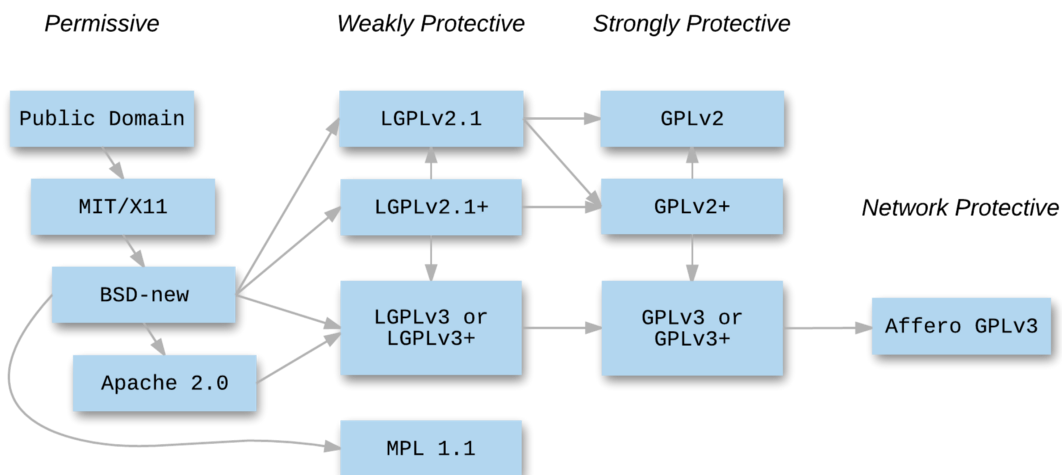
\includegraphics[width=0.9\textwidth]{c_licencias}
	\caption[Compatibilidad entre licencias]{Compatibilidad entre licencias~\cite{licencias}.}
	\label{fig:c_licencias}
\end{figure}

Como se puede observar en la figura anterior, podemos aplicar cualquier licencia a nuestro proyecto respecto a las dependencias que tenemos.

Se ha optado por: 

\textbf{GNU General Public License v3.0}\

<<Exige la publicación del código fuente y que todos los trabajos derivados del original conserven la misma licencia GPL, no permite enlaces con módulos privativos (de código cerrado) y requiere que todos los cambios realizados a la versión original sean reflejados en el código fuente con sus respectivos autores.
Los derechos de autor deben conservarse tanto en el código fuente como en los binarios.>>~\cite{GNU}

\subsubsection{Política de \emph{Cookies}}

El desarrollo de la aplicación ha implicado el uso de sesiones y por consiguiente, el uso de \emph{Cookies}. 

Las obligaciones legales de las \emph{cookies} se encuentran en: el artículo 22.2 LSSI (Ley de Servicios de la Sociedad de la Información y de Comercio Electrónico), este sentido el Grupo de Trabajo del Artículo 29 en su Dictamen 4/2012, indica que, quedan exceptuadas las que tienen por finalidad:

\begin{itemize}

\item\emph{Cookies} de entrada del usuario.
\item\emph{Cookies} de autenticación o identificación de usuario (únicamente de sesión)
\item\emph{Cookies} de seguridad del usuario
\item\emph{Cookies} de sesión de reproductor multimedia
\item\emph{Cookies} de sesión para equilibrar la carga
\item\emph{Cookies} de personalización de la interfaz de usuario
\item\emph{Cookies} de complemento (\emph{plugin}) para intercambiar contenidos sociales

\end{itemize}

En este caso, no es necesario informar, las que usa la aplicación \emph{SurveyingPointCode} son de tipo:

<<\emph{Cookies} de autenticación o identificación de usuario (únicamente de sesión).>>

Aun así se ha implementado un mensaje informando de que se está utilizando \emph{cookies} y cual es su uso.

El mensaje es el siguiente:
 
\begin{figure}[H]
	\centering
	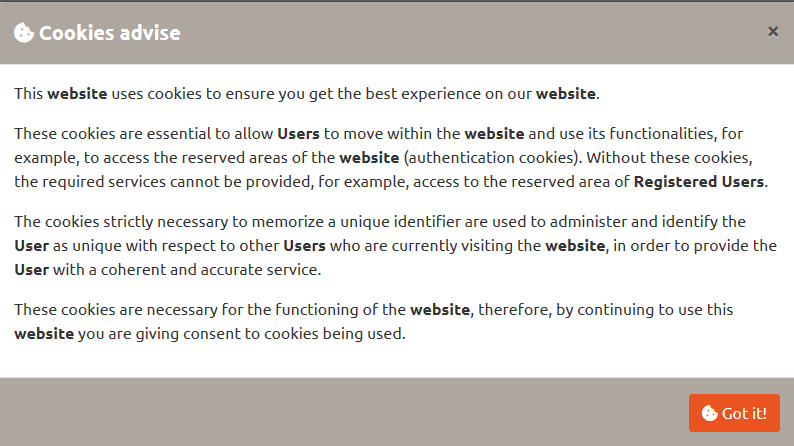
\includegraphics[width=1\textwidth]{cookies}
	\caption{Mensaje de aviso de \emph{Cookies}.}
	\label{fig:Scrum}
\end{figure}

\subsubsection{Uso de la dirección de e-mail}

En la aplicación se ha utilizado y registrado el dato del e-mail, para poder registrar y permitir el acceso del usuario. Este dato se considera de carácter personal, ya que hay ocasiones en que este se puede rastrear hasta conocer la identidad de la persona. Todo esto está regulado el la nueva Ley Orgánica de Protección de Datos de Carácter Personal 2018 \cite{LOPD}, donde se indica que el usuario debe aceptar el uso de su e-mail, debiendo ser el consentimiento explícito, específico y verificable y ese consentimiento ha de ser revocable en cualquier momento.

En este proyecto, al ser educacional no se han implementado esas opciones. Con este apartado se desea dejar claro que se está en conocimiento de la ley y de como aplicarla.


\subsubsection{Licencia en la documentación}

Con respecto a la documentación se ha optado por una licencia de tipo \emph{Creative Commons} y se ha elegido la siguiente:

\textbf{CC BY-NC-SA 4.0}~\cite{creativec}

Esta licencia permite a otros entremezclar, ajustar y construir a partir de su obra con fines no comerciales, siempre y cuando le reconozcan la autoría y sus nuevas creaciones estén bajo una licencia con los mismos términos.


\apendice{Especificación de Requisitos}

\section{Introducción}

En este anexo se describen los servicios que ha de ofrecer la aplicación \emph{SurveyingPointCode} y las restricciones asociadas a su funcionamiento. La función principal de la especificación de requisitos es servir como medio de comunicación entre clientes, usuarios, y desarrolladores.

Se recogerán todos los requisitos funcionales y no funcionales.

\section{Objetivos generales}
En este apartado se detallarán los distintos objetivos generales que se persiguen con este proyecto:

\begin{itemize}
\item Definir una codificación de puntos en un levantamiento topográfico que permita la automatización del proceso e delineación y mejore la toma de datos en campo.
\item Desarrollar una aplicación Web, que permita la conversión de un archivo de campo, con datos topográficos a un archivo DXF, interpretando la codificación y generando todos los elementos del dibujo de forma automática.
\item Trabajar con archivos personalizados del usuario como: configuración de la conversión y archivo DXF de símbolos, para la obtención del DXF final.
\item El usuario debe estar registrado, para acceder a la aplicación.
\end{itemize}

\section{Catalogo de requisitos}

A continuación,  definirán tanto los requisitos funcionales como los no
funcionales necesarios para cumplir con los objetivos generales.

\subsection{Requisitos funcionales}

\begin{itemize}
\item \textbf{RF-1 Registro de usuario: }el usuario debe poder 		registrarse, mediante un nombre, un e-mail y una contraseña.

\item \textbf{RF-2 \emph{Login} de usuario: }el usuario debe poder 	\emph{logearse}, mediante un e-mail y una contraseña.



\item \textbf{RF-3 Carga de archivos: }el usuario debe ser capaz de gestionar diferentes tipos de archivos: de campo, de configuración de la conversión y de símbolos.

\begin{itemize}
\item \textbf{RF-3.1 Carga de archivo de campo: }el usuario debe poder cargar este archivo con los datos de un levantamiento topográfico, indicando su validez y en caso contrario, indicando cual es su error. Este archivo es obligatorio.

\item \textbf{RF-3.2 Carga de archivo de configuración: }el usuario debe poder cargar este archivo con los datos de una configuración personalizada para la conversión, indicando su validez y en caso contrario, indicando cual es su error. Este archivo es opcional.

\item \textbf{RF-3.3 Carga de archivo DXF con simbología: }el usuario debe poder cargar este archivo DXF con símbolos personalizados, indicando su validez y en caso contrario, indicando cual es su error. Este archivo es opcional.
	
\end{itemize}

\item \textbf{RF-4 Conversión: }el usuario debe ser capaz de generar un archivo DXF, partiendo del archivo de campo, pudiendo configurar esa conversión utilizando los archivos opcionales. Debe también existir la posibilidad de configurar desde cero o modificar una configuración de la conversión existente a través de la interfaz gráfica. El usuario debe poder elegir la versión de CAD para el DXF a generar, y ponerle un nombre personalizado al archivo generado.

\begin{itemize}

\item \textbf{RF-4.1 Asociar capas y colores: }el usuario debe poder asociar capas y colores, a los códigos, a través del archivo configuración de la conversión o de la interfaz. 

\item \textbf{RF-4.2 Asociar símbolos: }el usuario debe poder asociar símbolos a los códigos. Previamente debe haber cargado un archivo válido con símbolos. 

\item \textbf{RF-4.3 Elección de versión de CAD: }el usuario debe poder elegir la versión de CAD para generar el DXF, a través de un desplegable con las versiones disponibles.

\item \textbf{RF-4.4 Elección de nombre del archivo DXF generado: }el usuario debe poder dar un nombre personalizado al archivo DXF generado.

\end{itemize}

\item \textbf{RF-5 Descarga de archivos :} el usuario debe poder descargar los archivos generados a su equipo de forma individual o varios archivos en formato comprimido.


\item \textbf{RF-6 \emph{Logout} del usuario: }el usuario debe poder cerrar la sesión.

\item \textbf{RF-7 Limpieza de archivos almacenados en el servidor: }la aplicación debe eliminar los archivos utilizados durante la sesión, al cerrarse la sesión.

\end{itemize}



\subsection{Requisitos no funcionales}

\begin{itemize}
\item \textbf{RNF-1 Usabilidad: }la aplicación debe ser intuitiva, con una curva baja de aprendizaje y mensajes de errores claros para el usuario.

\item \textbf{RNF-2 Soporte: }la aplicación debe funcionar en los navegadores Web más usuales, como: Google Chrome, Mozilla Firefox y Microsoft Edge.

\item \textbf{RNF-3 Rendimiento: }la aplicación debe tener unos tiempos de conversión del archivo mínimos, por ejemplo, con archivos de campo de tamaño grande, 5.000 puntos, debe realizar la conversión en no más de 5 segundos.

\item \textbf{RNF-4 Escalabilidad: }la aplicación debe ser desarrollada de manera que permita la escalabilidad de la misma de forma sencilla.

\item \textbf{RNF-5 Seguridad:} la aplicación debe gestionar de forma adecuada todos los datos sensibles, como claves, tokens, etc.

\end{itemize}

\section{Especificación de requisitos}

A continuación se mostrarán los diagramas de casos de uso y el detalle de cada uno de ellos.


\subsection{Actores}

En este sistema, existe un actor que interactuará con el sistema, y el propio sistema.


\subsection{Casos de uso}
\begin{figure}[H]
	\centering
	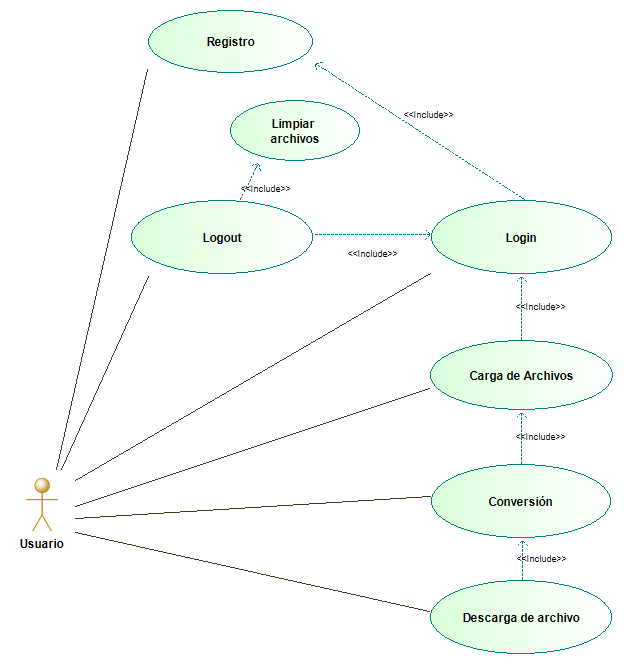
\includegraphics[width=1\textwidth]{CU-0}
	\caption{Diagrama de general de casos de uso.}
	\label{fig:CU-0}
\end{figure}


\imagen{CU-1}{Diagrama de caso de uso CU-01}
\strut
\begin{longtable}[H]{@{}ll@{}}
\toprule
\begin{minipage}[b]{0.23\columnwidth}\raggedright\strut
\textbf{CU-01}\strut
\end{minipage} & \begin{minipage}[b]{0.71\columnwidth}\raggedright\strut
\textbf{Registro del usuario}\strut
\end{minipage}\tabularnewline
\midrule
\endhead
\begin{minipage}[t]{0.23\columnwidth}\raggedright\strut
\textbf{Versión}\strut
\end{minipage} & \begin{minipage}[t]{0.71\columnwidth}\raggedright\strut
1.0\strut
\end{minipage}\tabularnewline
\begin{minipage}[t]{0.23\columnwidth}\raggedright\strut
\textbf{Autor}\strut
\end{minipage} & \begin{minipage}[t]{0.71\columnwidth}\raggedright\strut
José Eduardo Risco Sánchez-Cortés\strut
\end{minipage}\tabularnewline
\begin{minipage}[t]{0.23\columnwidth}\raggedright\strut
\textbf{Requisitos asociados}\strut
\end{minipage} & \begin{minipage}[t]{0.71\columnwidth}\raggedright\strut
RF-1\strut
\end{minipage}\tabularnewline
\begin{minipage}[t]{0.23\columnwidth}\raggedright\strut
\textbf{Descripción}\strut
\end{minipage} & \begin{minipage}[t]{0.71\columnwidth}\raggedright\strut
Permite al usuario registrarse.\strut
\end{minipage}\tabularnewline
\begin{minipage}[t]{0.23\columnwidth}\raggedright\strut
\textbf{Precondición}\strut
\end{minipage} & \begin{minipage}[t]{0.71\columnwidth}\raggedright\strut
El usuario no debe estar \emph{logeado}.\strut
\end{minipage}\tabularnewline
\begin{minipage}[t]{0.23\columnwidth}%\raggedright\strut
\textbf{Acciones}\strut
\end{minipage} & \begin{minipage}[t]{0.71\columnwidth}%\raggedright\strut
\begin{enumerate}
\def\labelenumi{\arabic{enumi}.}
\tightlist
\item
  El usuario entra en la aplicación y accede a la página de registro.
\item
  Introduce su nombre, e-mail, contraseña y confirma esta.
\item
  El usuario confirma el registro con el botón \emph{Register}
\end{enumerate}\strut
\end{minipage}\tabularnewline
\begin{minipage}[t]{0.23\columnwidth}%\raggedright\strut
\textbf{Postcondición}\strut
\end{minipage} & \begin{minipage}[t]{0.71\columnwidth}%\raggedright\strut
\begin{itemize}
\tightlist
\item
  La aplicación va a la pantalla de \emph{Login}
\item
  mensaje: \textit{You are now a registered user!}.
\end{itemize}\strut

\end{minipage}\tabularnewline
\begin{minipage}[t]{0.23\columnwidth}\raggedright\strut
\textbf{Excepciones}\strut
\end{minipage} & \begin{minipage}[t]{0.71\columnwidth}%\raggedright\strut
\begin{itemize}
\tightlist
\item
  mensaje: \textit{Please use a different username.}
\item
  mensaje: \textit{Please use a different email address.}
\item
  mensaje: \textit{Field must be equal to password.}  
  
\end{itemize}\strut
\end{minipage}\tabularnewline
\begin{minipage}[t]{0.23\columnwidth}\raggedright\strut
\textbf{Importancia}\strut
\end{minipage} & \begin{minipage}[t]{0.71\columnwidth}\raggedright\strut
Alta\strut
\end{minipage}\tabularnewline
\bottomrule
\caption{CU-01 Registro de usuarios.}
\end{longtable}

\strut\strut
\

\begin{figure}[H]
	\centering
	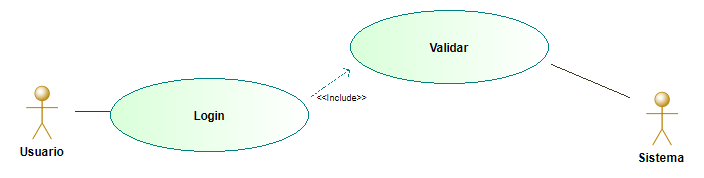
\includegraphics[width=1\textwidth]{CU-2}
	\caption{Diagrama de caso de uso CU-02.}
	\label{fig:CU-2}
\end{figure}

\strut
\begin{longtable}[H]{@{}ll@{}}
\toprule
\begin{minipage}[b]{0.23\columnwidth}\raggedright\strut
\textbf{CU-02}\strut
\end{minipage} & \begin{minipage}[b]{0.71\columnwidth}\raggedright\strut
\textbf{\emph{Login} de usuario}\strut
\end{minipage}\tabularnewline
\midrule
\endhead
\begin{minipage}[t]{0.23\columnwidth}\raggedright\strut
\textbf{Versión}\strut
\end{minipage} & \begin{minipage}[t]{0.71\columnwidth}\raggedright\strut
1.0\strut
\end{minipage}\tabularnewline
\begin{minipage}[t]{0.23\columnwidth}\raggedright\strut
\textbf{Autor}\strut
\end{minipage} & \begin{minipage}[t]{0.71\columnwidth}\raggedright\strut
José Eduardo Risco Sánchez-Cortés\strut
\end{minipage}\tabularnewline
\begin{minipage}[t]{0.23\columnwidth}\raggedright\strut
\textbf{Requisitos asociados}\strut
\end{minipage} & \begin{minipage}[t]{0.71\columnwidth}\raggedright\strut
RF-2\strut
\end{minipage}\tabularnewline
\begin{minipage}[t]{0.23\columnwidth}\raggedright\strut
\textbf{Descripción}\strut
\end{minipage} & \begin{minipage}[t]{0.71\columnwidth}\raggedright\strut
Permite al usuario \emph{logearse}.\strut
\end{minipage}\tabularnewline
\begin{minipage}[t]{0.23\columnwidth}\raggedright\strut
\textbf{Precondición}\strut
\end{minipage} & \begin{minipage}[t]{0.71\columnwidth}\raggedright\strut
El usuario debe estar registrado.\strut
\end{minipage}\tabularnewline
\begin{minipage}[t]{0.23\columnwidth}\raggedright\strut
\textbf{Acciones}\strut
\end{minipage} & \begin{minipage}[t]{0.71\columnwidth}\raggedright\strut
\begin{enumerate}
\def\labelenumi{\arabic{enumi}.}
\tightlist
\item
  El usuario entra en la aplicación y accede a la página de \emph{login}.
\item
  Introduce su e-mail y contraseña.
\item
  El usuario confirma el \emph{login} con el botón \emph{Submit}
\end{enumerate}\strut
\end{minipage}\tabularnewline
\begin{minipage}[t]{0.23\columnwidth}\raggedright\strut
\textbf{Postcondición}\strut
\end{minipage} & \begin{minipage}[t]{0.71\columnwidth}\raggedright\strut
La aplicación va a la pantalla de \emph{Upload File}
\end{minipage}\tabularnewline
\begin{minipage}[t]{0.23\columnwidth}\raggedright\strut
\textbf{Excepciones}\strut
\end{minipage} & \begin{minipage}[t]{0.71\columnwidth}\raggedright\strut
\begin{itemize}
\tightlist
\item
  mensaje: \textit{Invalid email address.}
\item
  mensaje: \textit{Invalid username or password!}
  
\end{itemize}\strut
\end{minipage}\tabularnewline
\begin{minipage}[t]{0.23\columnwidth}\raggedright\strut
\textbf{Importancia}\strut
\end{minipage} & \begin{minipage}[t]{0.71\columnwidth}\raggedright\strut
Alta\strut
\end{minipage}\tabularnewline
\bottomrule
\caption{CU-02 \emph{Login} de usuarios.}
\end{longtable}
\strut


\begin{figure}[H]
	\centering
	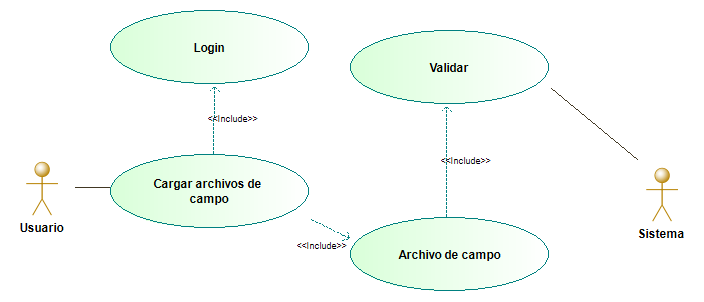
\includegraphics[width=0.7\textwidth]{CU-3}
	\caption{Diagrama de caso de uso CU-03.}
	\label{fig:CU-3}
\end{figure}
\begin{longtable}[H]{@{}ll@{}}
\toprule
\begin{minipage}[b]{0.23\columnwidth}\raggedright\strut
\textbf{CU-03}\strut
\end{minipage} & \begin{minipage}[b]{0.71\columnwidth}\raggedright\strut
\textbf{Carga de archivo de campo}\strut
\end{minipage}\tabularnewline
\midrule
\endhead
\begin{minipage}[t]{0.23\columnwidth}\raggedright\strut
\textbf{Versión}\strut
\end{minipage} & \begin{minipage}[t]{0.71\columnwidth}\raggedright\strut
1.0\strut
\end{minipage}\tabularnewline
\begin{minipage}[t]{0.23\columnwidth}\raggedright\strut
\textbf{Autor}\strut
\end{minipage} & \begin{minipage}[t]{0.71\columnwidth}\raggedright\strut
José Eduardo Risco Sánchez-Cortés\strut
\end{minipage}\tabularnewline
\begin{minipage}[t]{0.23\columnwidth}\raggedright\strut
\textbf{Requisitos asociados}\strut
\end{minipage} & \begin{minipage}[t]{0.71\columnwidth}\raggedright\strut
RF-3,RF-3.1, RF-2\strut
\end{minipage}\tabularnewline
\begin{minipage}[t]{0.23\columnwidth}\raggedright\strut
\textbf{Descripción}\strut
\end{minipage} & \begin{minipage}[t]{0.71\columnwidth}\raggedright\strut
Permite al usuario cargar un archivo de campo.\strut
\end{minipage}\tabularnewline
\begin{minipage}[t]{0.23\columnwidth}\raggedright\strut
\textbf{Precondición}\strut
\end{minipage} & \begin{minipage}[t]{0.71\columnwidth}\raggedright\strut
El usuario debe estar logeado.\\
El archivo debe tener extensión \texttt{txt} o \texttt{csv}.

\end{minipage}\tabularnewline
\begin{minipage}[t]{0.23\columnwidth}\raggedright\strut
\textbf{Acciones}\strut
\end{minipage} & \begin{minipage}[t]{0.71\columnwidth}%\raggedright\strut
\begin{enumerate}
\def\labelenumi{\arabic{enumi}.}
\tightlist
\item
  El usuario selecciona el archivo de campo, bien a través del botón \emph{Browse}, o arrastrando el archivo hasta la caja \emph{Topographical File data}.
\item
  El nombre del archivo aparece en la caja \emph{Topographical File data}.
\item
  El usuario confirma la carga con el botón \emph{Upload}
\end{enumerate}%\strut
\end{minipage}\tabularnewline
\begin{minipage}[t]{0.23\columnwidth}\raggedright\strut
\textbf{Postcondición}\strut
\end{minipage} & \begin{minipage}[t]{0.71\columnwidth}\raggedright\strut
La aplicación cambia a la pantalla de \emph{Upload File}
\end{minipage}\tabularnewline
\begin{minipage}[t]{0.23\columnwidth}%\raggedright\strut
\textbf{Excepciones}\strut
\end{minipage} & \begin{minipage}[t]{0.71\columnwidth}%\raggedright\strut
\begin{itemize}
\tightlist
\item
  mensaje: \textit{Topographic data file has the following errors...}
\item
  mensaje: \textit{Topographic data file is empty.}
\item
  mensaje: \textit{The number of points with \textit{TC} code in the topographic data file is not multiple of 2.}  
\item
  mensaje: \textit{The number of points with \textit{TR} code in the topographic data file is not multiple of 3.}  
\end{itemize}\strut
\end{minipage}\tabularnewline
\begin{minipage}[t]{0.23\columnwidth}%\raggedright\strut
\textbf{Importancia}\strut
\end{minipage} & \begin{minipage}[t]{0.71\columnwidth}%\raggedright\strut
Alta\strut
\end{minipage}\tabularnewline
\bottomrule
\caption{CU-03 Carga de archivo de campo.}
\end{longtable}


\imagen{CU-4}{Diagrama de caso de uso CU-04}

\begin{longtable}[H]{@{}ll@{}}
\toprule
\begin{minipage}[b]{0.23\columnwidth}\raggedright\strut
\textbf{CU-04}\strut
\end{minipage} & \begin{minipage}[b]{0.71\columnwidth}\raggedright\strut
\textbf{Carga de archivo de configuración}\strut
\end{minipage}\tabularnewline
\midrule
\endhead
\begin{minipage}[t]{0.23\columnwidth}\raggedright\strut
\textbf{Versión}\strut
\end{minipage} & \begin{minipage}[t]{0.71\columnwidth}\raggedright\strut
1.0\strut
\end{minipage}\tabularnewline
\begin{minipage}[t]{0.23\columnwidth}\raggedright\strut
\textbf{Autor}\strut
\end{minipage} & \begin{minipage}[t]{0.71\columnwidth}\raggedright\strut
José Eduardo Risco Sánchez-Cortés\strut
\end{minipage}\tabularnewline
\begin{minipage}[t]{0.23\columnwidth}\raggedright\strut
\textbf{Requisitos asociados}\strut
\end{minipage} & \begin{minipage}[t]{0.71\columnwidth}\raggedright\strut
RF-3,RF-3.1,RF-3.2, RF-2\strut
\end{minipage}\tabularnewline
\begin{minipage}[t]{0.23\columnwidth}\raggedright\strut
\textbf{Descripción}\strut
\end{minipage} & \begin{minipage}[t]{0.71\columnwidth}\raggedright\strut
Permite al usuario cargar un archivo de configuración de la conversión.\strut
\end{minipage}\tabularnewline
\begin{minipage}[t]{0.23\columnwidth}\raggedright\strut
\textbf{Precondición}\strut
\end{minipage} & \begin{minipage}[t]{0.71\columnwidth}\raggedright\strut
El usuario debe estar logeado.\\
El archivo debe tener extensión \texttt{txt} o \texttt{csv}.\\
El archivo de campo debe estar seleccionado

\end{minipage}\tabularnewline
\begin{minipage}[t]{0.23\columnwidth}\raggedright\strut
\textbf{Acciones}\strut
\end{minipage} & \begin{minipage}[t]{0.71\columnwidth}\raggedright\strut
\begin{enumerate}
\def\labelenumi{\arabic{enumi}.}
\tightlist
\item
  El usuario selecciona el archivo de configuración, bien a través del botón \emph{Browse}, o arrastrando el archivo hasta la caja \emph{User Configuration File}.
\item
  El nombre del archivo aparece en la caja \emph{User Configuration File}.
\item
  El usuario confirma la carga con el botón \emph{Upload}
   
\end{enumerate}\strut
\end{minipage}\tabularnewline
\begin{minipage}[t]{0.23\columnwidth}\raggedright\strut
\textbf{Postcondición}\strut
\end{minipage} & \begin{minipage}[t]{0.71\columnwidth}\raggedright\strut
\begin{enumerate}
\def\labelenumi{\arabic{enumi}.}
\tightlist
\item Postcondición 1, no se muestran errores:
La aplicación cambia a la pantalla de \emph{Upload File}\\
Aparece cargada la configuración en la tabla de la interfaz.\\
\item Postcondición 2, e muestran errores:
La aplicación cambia a la pantalla de \emph{Upload File}\\
Aparece cargada la configuración en la tabla de la interfaz.\\
Pueden mostrarse estos 2 errores:
\begin{itemize}
\tightlist
\item
  mensaje: \textit{User configuration has different colors on the same lines.}  
\item
  mensaje: \textit{Some color of the user configuration is not a CAD color.}      
\end{itemize}\strut  
Estos errores se deben subsanar por parte del usuario en esta pantalla sin necesidad de volver a cargar el archivo.
   
\end{enumerate}\strut


\end{minipage}\tabularnewline
\begin{minipage}[t]{0.23\columnwidth}\raggedright\strut
\textbf{Excepciones}\strut
\end{minipage} & \begin{minipage}[t]{0.71\columnwidth}\raggedright\strut
\begin{itemize}
\tightlist
\item
  mensaje: \textit{User configuration file file has the following errors...}
\item
  mensaje: \textit{User configuration file is empty.}
\item
  mensaje: \textit{User configuration file has duplicate items on different lines.}  

  
\end{itemize}\strut
\end{minipage}\tabularnewline
\begin{minipage}[t]{0.23\columnwidth}\raggedright\strut
\textbf{Importancia}\strut
\end{minipage} & \begin{minipage}[t]{0.71\columnwidth}\raggedright\strut
Alta\strut
\end{minipage}\tabularnewline
\bottomrule
\caption{CU-04 Carga de archivo de configuración.}
\end{longtable}

\begin{figure}[H]
	\centering
	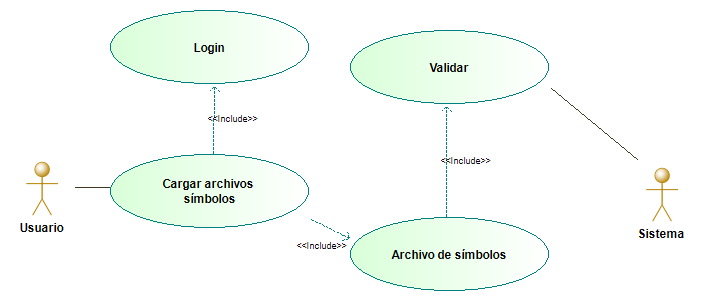
\includegraphics[width=0.7\textwidth]{CU-5}
	\caption{Diagrama de caso de uso CU-05.}
	\label{fig:CU-5}
\end{figure}

%\imagen{CU-5}{Diagrama de caso de uso CU-05}

\begin{longtable}[H]{@{}ll@{}}
\toprule
\begin{minipage}[b]{0.23\columnwidth}\raggedright\strut
\textbf{CU-05}\strut
\end{minipage} & \begin{minipage}[b]{0.71\columnwidth}\raggedright\strut
\textbf{Carga de archivo de símbolos}\strut
\end{minipage}\tabularnewline
\midrule
\endhead
\begin{minipage}[t]{0.23\columnwidth}\raggedright\strut
\textbf{Versión}\strut
\end{minipage} & \begin{minipage}[t]{0.71\columnwidth}\raggedright\strut
1.0\strut
\end{minipage}\tabularnewline
\begin{minipage}[t]{0.23\columnwidth}\raggedright\strut
\textbf{Autor}\strut
\end{minipage} & \begin{minipage}[t]{0.71\columnwidth}\raggedright\strut
José Eduardo Risco Sánchez-Cortés\strut
\end{minipage}\tabularnewline
\begin{minipage}[t]{0.23\columnwidth}\raggedright\strut
\textbf{Requisitos asociados}\strut
\end{minipage} & \begin{minipage}[t]{0.71\columnwidth}\raggedright\strut
RF-3, RF-3.1, RF-3.3, RF-2\strut
\end{minipage}\tabularnewline
\begin{minipage}[t]{0.23\columnwidth}\raggedright\strut
\textbf{Descripción}\strut
\end{minipage} & \begin{minipage}[t]{0.71\columnwidth}\raggedright\strut
Permite al usuario cargar un archivo DXF con símbolos.\strut
\end{minipage}\tabularnewline
\begin{minipage}[t]{0.23\columnwidth}\raggedright\strut
\textbf{Precondición}\strut
\end{minipage} & \begin{minipage}[t]{0.71\columnwidth}\raggedright\strut
El usuario debe estar logeado.\\
El archivo debe tener extensión \texttt{dxf}.\\
El archivo de campo debe estar seleccionado

\end{minipage}\tabularnewline
\begin{minipage}[t]{0.23\columnwidth}\raggedright\strut
\textbf{Acciones}\strut
\end{minipage} & \begin{minipage}[t]{0.71\columnwidth}\raggedright\strut
\begin{enumerate}
\def\labelenumi{\arabic{enumi}.}
\tightlist
\item
  El usuario selecciona el archivo de símbolos, bien a través del botón \emph{Browse}, o arrastrando el archivo hasta la caja \emph{CAD Symbols File}.
\item
  El nombre del archivo aparece en la caja \emph{CAD Symbols File}.
\item
  El usuario confirma la carga con el botón \emph{Upload}
\end{enumerate}\strut
\end{minipage}\tabularnewline
\begin{minipage}[t]{0.23\columnwidth}\raggedright
\textbf{Postcondición}\strut
\end{minipage} & \begin{minipage}[t]{0.71\columnwidth}\raggedright\strut
La aplicación cambia a la pantalla de \emph{Upload File}
\end{minipage}\tabularnewline
\begin{minipage}[t]{0.23\columnwidth}\raggedright\strut
\textbf{Excepciones}
\end{minipage} & \begin{minipage}[t]{0.71\columnwidth}%\raggedright\strut
\begin{itemize}
\tightlist
\item
  mensaje: \textit{CAD symbols file does not contain blocks.}

\end{itemize}\strut
\end{minipage}\tabularnewline
\begin{minipage}[t]{0.23\columnwidth}\raggedright\strut
\textbf{Importancia}\strut
\end{minipage} & \begin{minipage}[t]{0.71\columnwidth}\raggedright\strut
Alta\strut
\end{minipage}\tabularnewline
\bottomrule
\caption{CU-05 Carga de archivo de símbolos.}
\end{longtable}

\begin{figure}[H]
	\centering
	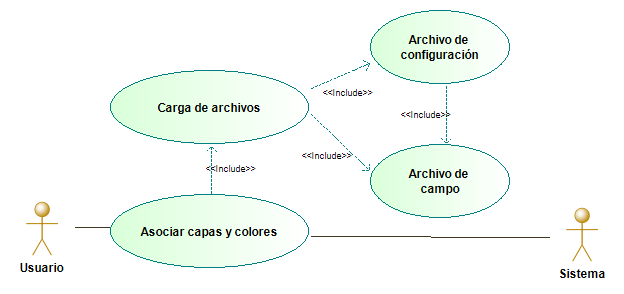
\includegraphics[width=0.7\textwidth]{CU-6}
	\caption{Diagrama de caso de uso CU-06.}
	\label{fig:CU-6}
\end{figure}


\begin{longtable}[H]{@{}ll@{}}
\toprule
\begin{minipage}[b]{0.23\columnwidth}\raggedright\strut
\textbf{CU-06}\strut
\end{minipage} & \begin{minipage}[b]{0.71\columnwidth}\raggedright\strut
\textbf{Asociar capas y colores}\strut
\end{minipage}\tabularnewline
\midrule
\endhead
\begin{minipage}[t]{0.23\columnwidth}\raggedright\strut
\textbf{Versión}\strut
\end{minipage} & \begin{minipage}[t]{0.71\columnwidth}\raggedright\strut
1.0\strut
\end{minipage}\tabularnewline
\begin{minipage}[t]{0.23\columnwidth}\raggedright\strut
\textbf{Autor}\strut
\end{minipage} & \begin{minipage}[t]{0.71\columnwidth}\raggedright\strut
José Eduardo Risco Sánchez-Cortés\strut
\end{minipage}\tabularnewline
\begin{minipage}[t]{0.23\columnwidth}\raggedright\strut
\textbf{Requisitos asociados}\strut
\end{minipage} & \begin{minipage}[t]{0.71\columnwidth}\raggedright\strut
RF-4, RF-4.1, RF-3, RF-3.1 \strut
\end{minipage}\tabularnewline
\begin{minipage}[t]{0.23\columnwidth}\raggedright\strut
\textbf{Descripción}\strut
\end{minipage} & \begin{minipage}[t]{0.71\columnwidth}\raggedright\strut
Permite al usuario asociar capas y colores, a los códigos extraídos del archivo de campo\strut
\end{minipage}\tabularnewline
\begin{minipage}[t]{0.23\columnwidth}\raggedright\strut
\textbf{Precondición}\strut
\end{minipage} & \begin{minipage}[t]{0.71\columnwidth}\raggedright\strut
El archivo de campo debe estar cargado.

\end{minipage}\tabularnewline
\begin{minipage}[t]{0.23\columnwidth}\raggedright\strut
\textbf{Acciones}\strut
\end{minipage} & \begin{minipage}[t]{0.71\columnwidth}\raggedright\strut
\begin{enumerate}
\def\labelenumi{\arabic{enumi}.}
\tightlist
\item
  El usuario introduce nombres de capas y selecciona colores, en la tabla, a través de la interfaz. En el caso de haber cargado un archivo de configuración esta aparecerá cargada en la tabla y se podrá modificar por el usuario.

\end{enumerate}\strut
\end{minipage}\tabularnewline
\begin{minipage}[t]{0.23\columnwidth}\raggedright\strut
\textbf{Postcondición}\strut
\end{minipage} & \begin{minipage}[t]{0.71\columnwidth}\raggedright\strut
  Los nombres de capas y colores seleccionados deben permanecer en la interfaz.
\end{minipage}\tabularnewline
\begin{minipage}[t]{0.23\columnwidth}\raggedright\strut
\textbf{Excepciones}\strut
\end{minipage} & \begin{minipage}[t]{0.71\columnwidth}\raggedright\strut
-\strut
\end{minipage}\tabularnewline
\begin{minipage}[t]{0.23\columnwidth}\raggedright\strut
\textbf{Importancia}\strut
\end{minipage} & \begin{minipage}[t]{0.71\columnwidth}\raggedright\strut
Alta\strut
\end{minipage}\tabularnewline
\bottomrule
\caption{CU-06 Asociar capas y colores.}
\end{longtable}
\strut
\imagen{CU-7}{Diagrama de caso de uso CU-07}
\strut
\begin{longtable}[H]{@{}ll@{}}
\toprule
\begin{minipage}[b]{0.23\columnwidth}\raggedright\strut
\textbf{CU-07}\strut
\end{minipage} & \begin{minipage}[b]{0.71\columnwidth}\raggedright\strut
\textbf{Asociar símbolos}\strut
\end{minipage}\tabularnewline
\midrule
\endhead
\begin{minipage}[t]{0.23\columnwidth}\raggedright\strut
\textbf{Versión}\strut
\end{minipage} & \begin{minipage}[t]{0.71\columnwidth}\raggedright\strut
1.0\strut
\end{minipage}\tabularnewline
\begin{minipage}[t]{0.23\columnwidth}\raggedright\strut
\textbf{Autor}\strut
\end{minipage} & \begin{minipage}[t]{0.71\columnwidth}\raggedright\strut
José Eduardo Risco Sánchez-Cortés\strut
\end{minipage}\tabularnewline
\begin{minipage}[t]{0.23\columnwidth}\raggedright\strut
\textbf{Requisitos asociados}\strut
\end{minipage} & \begin{minipage}[t]{0.71\columnwidth}\raggedright\strut
RF-4, RF-4.2, RF-3, RF-3.1\strut
\end{minipage}\tabularnewline
\begin{minipage}[t]{0.23\columnwidth}\raggedright\strut
\textbf{Descripción}\strut
\end{minipage} & \begin{minipage}[t]{0.71\columnwidth}\raggedright\strut
Permite al usuario asociar símbolos, a los códigos extraídos del archivo de campo\strut
\end{minipage}\tabularnewline
\begin{minipage}[t]{0.23\columnwidth}\raggedright\strut
\textbf{Precondición}\strut
\end{minipage} & \begin{minipage}[t]{0.71\columnwidth}\raggedright\strut
El archivo de campo debe estar cargado.\\
El archivo de símbolos debe estar cargado.

\end{minipage}\tabularnewline
\begin{minipage}[t]{0.23\columnwidth}\raggedright\strut
\textbf{Acciones}\strut
\end{minipage} & \begin{minipage}[t]{0.71\columnwidth}\raggedright\strut
\begin{enumerate}
\def\labelenumi{\arabic{enumi}.}
\tightlist
\item
 El usuario elige el símbolo a asociar a cada capa mediante un botón desplegable que contienen todos los símbolos disponibles.

\end{enumerate}\strut
\end{minipage}\tabularnewline
\begin{minipage}[t]{0.23\columnwidth}\raggedright\strut
\textbf{Postcondición}\strut
\end{minipage} & \begin{minipage}[t]{0.71\columnwidth}\raggedright\strut
  Los símbolos elegidos deben permanecer en la interfaz.
\end{minipage}\tabularnewline
\begin{minipage}[t]{0.23\columnwidth}\raggedright\strut
\textbf{Excepciones}\strut
\end{minipage} & \begin{minipage}[t]{0.71\columnwidth}\raggedright\strut
-\strut
\end{minipage}\tabularnewline
\begin{minipage}[t]{0.23\columnwidth}\raggedright\strut
\textbf{Importancia}\strut
\end{minipage} & \begin{minipage}[t]{0.71\columnwidth}\raggedright\strut
Alta\strut
\end{minipage}\tabularnewline
\bottomrule
\caption{CU-07 Asociar símbolos.}
\end{longtable}
\newpage

\begin{figure}[H]
	\centering
	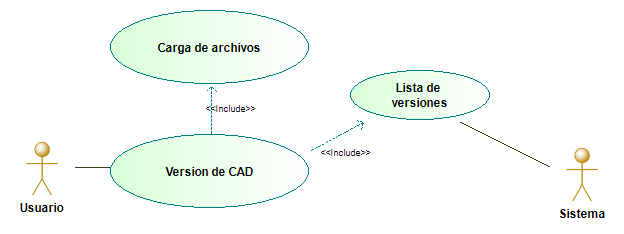
\includegraphics[width=1\textwidth]{CU-8}
	\caption{Diagrama de caso de uso CU-08.}
	\label{fig:CU-8}
\end{figure}


\strut

\begin{longtable}[H]{@{}ll@{}}
\toprule
\begin{minipage}[b]{0.23\columnwidth}\raggedright\strut
\textbf{CU-08}\strut
\end{minipage} & \begin{minipage}[b]{0.71\columnwidth}\raggedright\strut
\textbf{Elegir versión de CAD}\strut
\end{minipage}\tabularnewline
\midrule
\endhead
\begin{minipage}[t]{0.23\columnwidth}\raggedright\strut
\textbf{Versión}\strut
\end{minipage} & \begin{minipage}[t]{0.71\columnwidth}\raggedright\strut
1.0\strut
\end{minipage}\tabularnewline
\begin{minipage}[t]{0.23\columnwidth}\raggedright\strut
\textbf{Autor}\strut
\end{minipage} & \begin{minipage}[t]{0.71\columnwidth}\raggedright\strut
José Eduardo Risco Sánchez-Cortés\strut
\end{minipage}\tabularnewline
\begin{minipage}[t]{0.23\columnwidth}\raggedright\strut
\textbf{Requisitos asociados}\strut
\end{minipage} & \begin{minipage}[t]{0.71\columnwidth}\raggedright\strut
RF-4, RF-4.3, RF-3, RF-3.1\strut
\end{minipage}\tabularnewline
\begin{minipage}[t]{0.23\columnwidth}\raggedright\strut
\textbf{Descripción}\strut
\end{minipage} & \begin{minipage}[t]{0.71\columnwidth}\raggedright\strut
Permite al usuario elegir la versión de CAD para el archivo DXF generado\strut
\end{minipage}\tabularnewline
\begin{minipage}[t]{0.23\columnwidth}\raggedright\strut
\textbf{Precondición}\strut
\end{minipage} & \begin{minipage}[t]{0.71\columnwidth}\raggedright\strut
El archivo de campo debe estar cargado.\\
Deben ser accesibles las versiones de CAD disponibles. 
\end{minipage}\tabularnewline
\begin{minipage}[t]{0.23\columnwidth}\raggedright\strut
\textbf{Acciones}\strut
\end{minipage} & \begin{minipage}[t]{0.71\columnwidth}\raggedright\strut
\begin{enumerate}
\def\labelenumi{\arabic{enumi}.}
\tightlist
\item
 El usuario elige la versión de CAD mediante un botón desplegable que contienen todos los símbolos disponibles.
\end{enumerate}\strut
\end{minipage}\tabularnewline
\begin{minipage}[t]{0.23\columnwidth}\raggedright\strut
\textbf{Postcondición}\strut
\end{minipage} & \begin{minipage}[t]{0.71\columnwidth}\raggedright\strut
  La versión elegida debe permanecer en la interfaz.
\end{minipage}\tabularnewline
\begin{minipage}[t]{0.23\columnwidth}\raggedright\strut
\textbf{Excepciones}\strut
\end{minipage} & \begin{minipage}[t]{0.71\columnwidth}\raggedright\strut
-\strut
\end{minipage}\tabularnewline
\begin{minipage}[t]{0.23\columnwidth}\raggedright\strut
\textbf{Importancia}\strut
\end{minipage} & \begin{minipage}[t]{0.71\columnwidth}\raggedright\strut
Alta\strut
\end{minipage}\tabularnewline
\bottomrule
\caption{CU-08 Elegir versión de CAD.}
\end{longtable}


\begin{figure}[H]
	\centering
	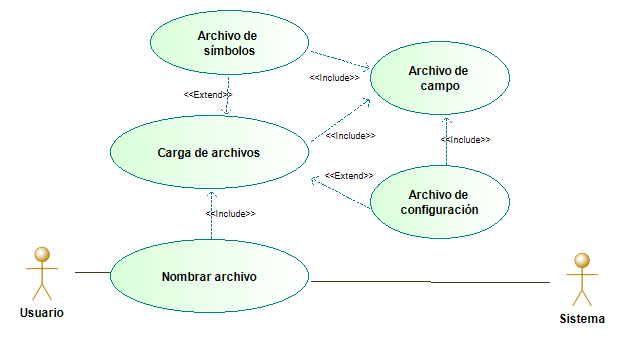
\includegraphics[width=1\textwidth]{CU-9}
	\caption{Diagrama de caso de uso CU-09.}
	\label{fig:CU-9}
\end{figure}

\strut
\begin{longtable}[H]{@{}ll@{}}
\toprule
\begin{minipage}[b]{0.23\columnwidth}\raggedright\strut
\textbf{CU-09}\strut
\end{minipage} & \begin{minipage}[b]{0.71\columnwidth}\raggedright\strut
\textbf{Dar nombre al archivo DXF generado}\strut
\end{minipage}\tabularnewline
\midrule
\endhead
\begin{minipage}[t]{0.23\columnwidth}\raggedright\strut
\textbf{Versión}\strut
\end{minipage} & \begin{minipage}[t]{0.71\columnwidth}\raggedright\strut
1.0\strut
\end{minipage}\tabularnewline
\begin{minipage}[t]{0.23\columnwidth}\raggedright\strut
\textbf{Autor}\strut
\end{minipage} & \begin{minipage}[t]{0.71\columnwidth}\raggedright\strut
José Eduardo Risco Sánchez-Cortés\strut
\end{minipage}\tabularnewline
\begin{minipage}[t]{0.23\columnwidth}\raggedright\strut
\textbf{Requisitos asociados}\strut
\end{minipage} & \begin{minipage}[t]{0.71\columnwidth}\raggedright\strut
RF-4, RF-4.4, RF-3, RF-3.1\strut
\end{minipage}\tabularnewline
\begin{minipage}[t]{0.23\columnwidth}\raggedright\strut
\textbf{Descripción}\strut
\end{minipage} & \begin{minipage}[t]{0.71\columnwidth}\raggedright\strut
Permite al usuario dar un nombre personalizado al archivo DXF generado\strut
\end{minipage}\tabularnewline
\begin{minipage}[t]{0.23\columnwidth}\raggedright\strut
\textbf{Precondición}\strut
\end{minipage} & \begin{minipage}[t]{0.71\columnwidth}\raggedright\strut
El archivo de campo debe estar cargado.\\
\end{minipage}\tabularnewline
\begin{minipage}[t]{0.23\columnwidth}\raggedright\strut
\textbf{Acciones}\strut
\end{minipage} & \begin{minipage}[t]{0.71\columnwidth}\raggedright\strut
\begin{enumerate}
\def\labelenumi{\arabic{enumi}.}
\tightlist
\item
 El usuario escribe un nombre en la caja llamada \emph{Filename }
\item
El nombre del archivo aparece en la caja.

\end{enumerate}\strut
\end{minipage}\tabularnewline
\begin{minipage}[t]{0.23\columnwidth}\raggedright\strut
\textbf{Postcondición}\strut
\end{minipage} & \begin{minipage}[t]{0.71\columnwidth}\raggedright\strut
El nombre del archivo debe permanecer en la interfaz.
\end{minipage}\tabularnewline
\begin{minipage}[t]{0.23\columnwidth}\raggedright\strut
\textbf{Excepciones}\strut
\end{minipage} & \begin{minipage}[t]{0.71\columnwidth}\raggedright\strut
-\strut
\end{minipage}\tabularnewline
\begin{minipage}[t]{0.23\columnwidth}\raggedright\strut
\textbf{Importancia}\strut
\end{minipage} & \begin{minipage}[t]{0.71\columnwidth}\raggedright\strut
Media\strut
\end{minipage}\tabularnewline
\bottomrule
\caption{CU-09 Dar nombre al archivo DXF generado.}
\end{longtable}

\newpage

\begin{figure}[H]
	\centering
	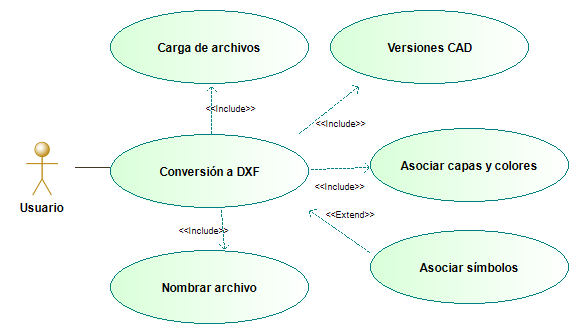
\includegraphics[width=0.7\textwidth]{CU-10}
	\caption{Diagrama de caso de uso CU-10.}
	\label{fig:CU-10}
\end{figure}


\begin{longtable}[H]{@{}ll@{}}
\toprule
\begin{minipage}[b]{0.23\columnwidth}\raggedright\strut
\textbf{CU-10}\strut
\end{minipage} & \begin{minipage}[b]{0.71\columnwidth}\raggedright\strut
\textbf{Conversión a DXF}\strut
\end{minipage}\tabularnewline
\midrule
\endhead
\begin{minipage}[t]{0.23\columnwidth}\raggedright\strut
\textbf{Versión}\strut
\end{minipage} & \begin{minipage}[t]{0.71\columnwidth}\raggedright\strut
1.0\strut
\end{minipage}\tabularnewline
\begin{minipage}[t]{0.23\columnwidth}\raggedright\strut
\textbf{Autor}\strut
\end{minipage} & \begin{minipage}[t]{0.71\columnwidth}\raggedright\strut
José Eduardo Risco Sánchez-Cortés\strut
\end{minipage}\tabularnewline
\begin{minipage}[t]{0.23\columnwidth}\raggedright\strut
\textbf{Requisitos asociados}\strut
\end{minipage} & \begin{minipage}[t]{0.71\columnwidth}\raggedright\strut
RF-4, RF-4.1,RF-4.2,RF-4.3, RF-4.4, RF-3, RF-3.1\, RF-3.2, RF-3.3\strut
\end{minipage}\tabularnewline
\begin{minipage}[t]{0.23\columnwidth}\raggedright\strut
\textbf{Descripción}\strut
\end{minipage} & \begin{minipage}[t]{0.71\columnwidth}\raggedright\strut
Permite al usuario generar un archivo DXF \strut
\end{minipage}\tabularnewline
\begin{minipage}[t]{0.23\columnwidth}\raggedright\strut
\textbf{Precondición}\strut
\end{minipage} & \begin{minipage}[t]{0.71\columnwidth}\raggedright\strut
El archivo de campo debe estar cargado.\\
\end{minipage}\tabularnewline
\begin{minipage}[t]{0.23\columnwidth}\raggedright\strut
\textbf{Acciones}\strut
\end{minipage} & \begin{minipage}[t]{0.71\columnwidth}\raggedright\strut
\begin{enumerate}
\def\labelenumi{\arabic{enumi}.}
\tightlist
\item
  El usuario confirma la conversión con el botón \emph{Convert}
\end{enumerate}\strut
\end{minipage}\tabularnewline
\begin{minipage}[t]{0.23\columnwidth}\raggedright\strut
\textbf{Postcondición}\strut
\end{minipage} & \begin{minipage}[t]{0.71\columnwidth}\raggedright\strut
La aplicación cambia a la pantalla de \emph{Download File}\\
mensaje: \emph{File successfully converted!}
\end{minipage}\tabularnewline
\begin{minipage}[t]{0.23\columnwidth}\raggedright\strut
\textbf{Excepciones}\strut
\end{minipage} & \begin{minipage}[t]{0.71\columnwidth}\raggedright\strut
\begin{itemize}
\tightlist

\item
  mensaje: \textit{User configuration file has duplicate items on different lines.}  
\item
  mensaje: \textit{User configuration has different colors on the same lines.} 

\end{itemize}\strut
\end{minipage}\tabularnewline
\begin{minipage}[t]{0.23\columnwidth}\raggedright\strut
\textbf{Importancia}\strut
\end{minipage} & \begin{minipage}[t]{0.71\columnwidth}\raggedright\strut
Alta\strut
\end{minipage}\tabularnewline
\bottomrule
\caption{CU-10 Conversión a DXF.}
\end{longtable}

\newpage

\begin{figure}[H]
	\centering
	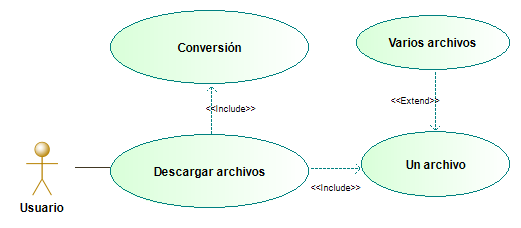
\includegraphics[width=0.7\textwidth]{CU-11}
	\caption{Diagrama de caso de uso CU-11.}
	\label{fig:CU-11}
\end{figure}

\begin{longtable}[H]{@{}ll@{}}
\toprule
\begin{minipage}[b]{0.23\columnwidth}\raggedright\strut
\textbf{CU-11}\strut
\end{minipage} & \begin{minipage}[b]{0.71\columnwidth}\raggedright\strut
\textbf{Descargar archivos}\strut
\end{minipage}\tabularnewline
\midrule
\endhead
\begin{minipage}[t]{0.23\columnwidth}\raggedright\strut
\textbf{Versión}\strut
\end{minipage} & \begin{minipage}[t]{0.71\columnwidth}\raggedright\strut
1.0\strut
\end{minipage}\tabularnewline
\begin{minipage}[t]{0.23\columnwidth}\raggedright\strut
\textbf{Autor}\strut
\end{minipage} & \begin{minipage}[t]{0.71\columnwidth}\raggedright\strut
José Eduardo Risco Sánchez-Cortés\strut
\end{minipage}\tabularnewline
\begin{minipage}[t]{0.23\columnwidth}\raggedright\strut
\textbf{Requisitos asociados}\strut
\end{minipage} & \begin{minipage}[t]{0.71\columnwidth}\raggedright\strut
RF-5, RF-4, RF-4.1,RF-4.2,RF-4.3, RF-4.4\strut
\end{minipage}\tabularnewline
\begin{minipage}[t]{0.23\columnwidth}\raggedright\strut
\textbf{Descripción}\strut
\end{minipage} & \begin{minipage}[t]{0.71\columnwidth}\raggedright\strut
Permite al usuario descargar a su equipo los archivos generados. \strut
\end{minipage}\tabularnewline
\begin{minipage}[t]{0.23\columnwidth}\raggedright\strut
\textbf{Precondición}\strut
\end{minipage} & \begin{minipage}[t]{0.71\columnwidth}\raggedright\strut
Deben existir archivos convertidos a DXF.\\
\end{minipage}\tabularnewline
\begin{minipage}[t]{0.23\columnwidth}\raggedright\strut
\textbf{Acciones}\strut
\end{minipage} & \begin{minipage}[t]{0.71\columnwidth}\raggedright
\begin{enumerate}
\def\labelenumi{\arabic{enumi}.}
\tightlist
\item
  El usuario puede elegir descargar un archivo individualmente.
\begin{itemize}
\tightlist
\item
  El usuario pulsa sobre el archivo a descargar. 
\item
  El archivo se descarga correctamente con formato dxf.
\end{itemize}
\item
  El usuario puede elegir descargar varios archivos a la vez.
\begin{itemize}
\tightlist
\item
  El usuario pulsa sobre el botón \emph{Download all}. 
\item
  El archivo se descarga correctamente con formato comprimido zip.
\end{itemize}
\end{enumerate}\strut
\end{minipage}\tabularnewline
\begin{minipage}[t]{0.23\columnwidth}\raggedright\strut
\textbf{Postcondición}\strut
\end{minipage} & \begin{minipage}[t]{0.71\columnwidth}\raggedright\strut
La aplicación permanece la pantalla de \emph{Download File}
\end{minipage}\tabularnewline
\begin{minipage}[t]{0.23\columnwidth}\raggedright\strut
\textbf{Excepciones}\strut
\end{minipage} & \begin{minipage}[t]{0.71\columnwidth}\raggedright\strut
-\strut
\end{minipage}\tabularnewline
\begin{minipage}[t]{0.23\columnwidth}\raggedright\strut
\textbf{Importancia}\strut
\end{minipage} & \begin{minipage}[t]{0.71\columnwidth}\raggedright\strut
Alta\strut
\end{minipage}\tabularnewline
\bottomrule
\caption{CU-11 Descargar archivos.}
\end{longtable}

\newpage


\imagen{CU-12}{Diagrama de caso de uso CU-12}

\begin{longtable}[H]{@{}ll@{}}
\toprule
\begin{minipage}[b]{0.23\columnwidth}\raggedright\strut
\textbf{CU-12}\strut
\end{minipage} & \begin{minipage}[b]{0.71\columnwidth}\raggedright\strut
\textbf{\emph{Logout}}\strut
\end{minipage}\tabularnewline
\midrule
\endhead
\begin{minipage}[t]{0.23\columnwidth}\raggedright\strut
\textbf{Versión}\strut
\end{minipage} & \begin{minipage}[t]{0.71\columnwidth}\raggedright\strut
1.0\strut
\end{minipage}\tabularnewline
\begin{minipage}[t]{0.23\columnwidth}\raggedright\strut
\textbf{Autor}\strut
\end{minipage} & \begin{minipage}[t]{0.71\columnwidth}\raggedright\strut
José Eduardo Risco Sánchez-Cortés\strut
\end{minipage}\tabularnewline
\begin{minipage}[t]{0.23\columnwidth}\raggedright\strut
\textbf{Requisitos asociados}\strut
\end{minipage} & \begin{minipage}[t]{0.71\columnwidth}\raggedright\strut
RF-6, RF-2\strut
\end{minipage}\tabularnewline
\begin{minipage}[t]{0.23\columnwidth}\raggedright\strut
\textbf{Descripción}\strut
\end{minipage} & \begin{minipage}[t]{0.71\columnwidth}\raggedright\strut
Permite al usuario cerrar la sesión. \strut
\end{minipage}\tabularnewline
\begin{minipage}[t]{0.23\columnwidth}\raggedright\strut
\textbf{Precondición}\strut
\end{minipage} & \begin{minipage}[t]{0.71\columnwidth}\raggedright\strut
El usuario debe estar \emph{logeado}.\\
\end{minipage}\tabularnewline
\begin{minipage}[t]{0.23\columnwidth}\raggedright\strut
\textbf{Acciones}\strut
\end{minipage} & \begin{minipage}[t]{0.71\columnwidth}\raggedright
\begin{enumerate}
\def\labelenumi{\arabic{enumi}.}
\tightlist
\item
  El usuario pulsa el botón \emph{Sign out}.
\item
  La aplicación va a la pantalla de bienvenida.

\end{enumerate}\strut
\end{minipage}\tabularnewline
\begin{minipage}[t]{0.23\columnwidth}\raggedright\strut
\textbf{Postcondición}\strut
\end{minipage} & \begin{minipage}[t]{0.71\columnwidth}\raggedright\strut
La aplicación cierra la sesión.
\end{minipage}\tabularnewline
\begin{minipage}[t]{0.23\columnwidth}\raggedright\strut
\textbf{Excepciones}\strut
\end{minipage} & \begin{minipage}[t]{0.71\columnwidth}\raggedright\strut
-\strut
\end{minipage}\tabularnewline
\begin{minipage}[t]{0.23\columnwidth}\raggedright\strut
\textbf{Importancia}\strut
\end{minipage} & \begin{minipage}[t]{0.71\columnwidth}\raggedright\strut
Alta\strut
\end{minipage}\tabularnewline
\bottomrule
\caption{CU-12 \emph{Logout}.}
\end{longtable}

\newpage

\imagen{CU-13}{Diagrama de caso de uso CU-13}

\begin{longtable}[H]{@{}ll@{}}
\toprule
\begin{minipage}[b]{0.23\columnwidth}\raggedright\strut
\textbf{CU-12}\strut
\end{minipage} & \begin{minipage}[b]{0.71\columnwidth}\raggedright\strut
\textbf{Limpiar archivos}\strut
\end{minipage}\tabularnewline
\midrule
\endhead
\begin{minipage}[t]{0.23\columnwidth}\raggedright\strut
\textbf{Versión}\strut
\end{minipage} & \begin{minipage}[t]{0.71\columnwidth}\raggedright\strut
1.0\strut
\end{minipage}\tabularnewline
\begin{minipage}[t]{0.23\columnwidth}\raggedright\strut
\textbf{Autor}\strut
\end{minipage} & \begin{minipage}[t]{0.71\columnwidth}\raggedright\strut
José Eduardo Risco Sánchez-Cortés\strut
\end{minipage}\tabularnewline
\begin{minipage}[t]{0.23\columnwidth}\raggedright\strut
\textbf{Requisitos asociados}\strut
\end{minipage} & \begin{minipage}[t]{0.71\columnwidth}\raggedright\strut
RF-7, RF-6, RF-2\strut
\end{minipage}\tabularnewline
\begin{minipage}[t]{0.23\columnwidth}\raggedright\strut
\textbf{Descripción}\strut
\end{minipage} & \begin{minipage}[t]{0.71\columnwidth}\raggedright\strut
Permite al sistema eliminar los archivos usados durante la sesión. \strut
\end{minipage}\tabularnewline
\begin{minipage}[t]{0.23\columnwidth}\raggedright\strut
\textbf{Precondición}\strut
\end{minipage} & \begin{minipage}[t]{0.71\columnwidth}\raggedright\strut
El usuario debe estar \emph{logeado}.\\
El usuario debe haber subido archivos o realizado conversiones.\\
\end{minipage}\tabularnewline
\begin{minipage}[t]{0.23\columnwidth}\raggedright\strut
\textbf{Acciones}\strut
\end{minipage} & \begin{minipage}[t]{0.71\columnwidth}\raggedright
\begin{enumerate}
\def\labelenumi{\arabic{enumi}.}
\tightlist
\item
  El usuario pulsa el botón \emph{Sign out}.
\item
  La aplicación va a la pantalla de bienvenida.

\end{enumerate}\strut
\end{minipage}\tabularnewline
\begin{minipage}[t]{0.23\columnwidth}\raggedright\strut
\textbf{Postcondición}\strut
\end{minipage} & \begin{minipage}[t]{0.71\columnwidth}\raggedright\strut
La aplicación elimina todos los archivos utilizados en la sesión.
\end{minipage}\tabularnewline
\begin{minipage}[t]{0.23\columnwidth}\raggedright\strut
\textbf{Excepciones}\strut
\end{minipage} & \begin{minipage}[t]{0.71\columnwidth}\raggedright\strut
-\strut
\end{minipage}\tabularnewline
\begin{minipage}[t]{0.23\columnwidth}\raggedright\strut
\textbf{Importancia}\strut
\end{minipage} & \begin{minipage}[t]{0.71\columnwidth}\raggedright\strut
Media\strut
\end{minipage}\tabularnewline
\bottomrule
\caption{CU-13 Limpiar archivos.}
\end{longtable}
\strut
\apendice{Especificación de diseño}

\section{Introducción}
En este apartado se describe cómo se ha diseñado la aplicación \emph{SurveyingPointCode} para cumplir con los objetivos y las especificaciones definidas anteriormente.

Se definen los datos a utilizar por la aplicación así como el diseño procedimental y su arquitectura.
\section{Diseño de datos}

Las entidades de esta aplicación están enfocadas a la generación de un dibujo final. A continuación se describe cuales son y como se relacionan entre ellas. 


\begin{itemize}

\item \textbf{Dibujo:} Almacena todos los elementos que componen el dibujo, tanto geométricos, como no geométricos. Está compuesto por: un nombre, capas, puntos y textos. De forma opcional puede contener: lineas, \emph{splines}, círculos y símbolos.

\item \textbf{Capa:} Todos los elementos del dibujo se guardan en capas. Está compuesto por: un nombre y un color.

\item \textbf{Punto:} Elemento básico del dibujo. Está compuesto por: un número, una coordenada $X$, una coordenada $Y$, una coordenada $Z$, un código y una capa.

\item \textbf{Línea:} Formada por una lista de puntos. Está compuesto por: una lista de puntos y una capa.

\item \textbf{\emph{spline}:} Formada por una lista de puntos. Está compuesto por: una lista de puntos y una capa.

\item \textbf{Círculo:} Está compuesto por: un punto, un radio y una capa.

\item \textbf{Bloque:} Elemento interno de CAD que almacena un símbolo. Está compuesto por: un nombre, un punto y una capa.

\item \textbf{Texto:} Texto asociado a un punto, en este caso pude ser, el número del punto, su altitud o su código. Está compuesto por: un punto, el tamaño del texto, el desplazamiento con respecto al punto, el texto y una capa.

\end{itemize}

Aunque no se ha implementado como una base de datos, la relación entre los elementos dentro de la biblioteca \texttt{ezdxf}, se comporta de la misma forma.

A continuación se puede ver el diagrama relacional. Se ha representado en dos diagramas para facilitar su comprensión (en un mismo diagrama saldrían líneas superpuestas y sería muy confuso de interpretar).

En la Figura~\ref{fig:DR-1}, se ven las relaciones de todos los elementos con el elemento principal , el dibujo.

\begin{figure}[H]
	\centering
	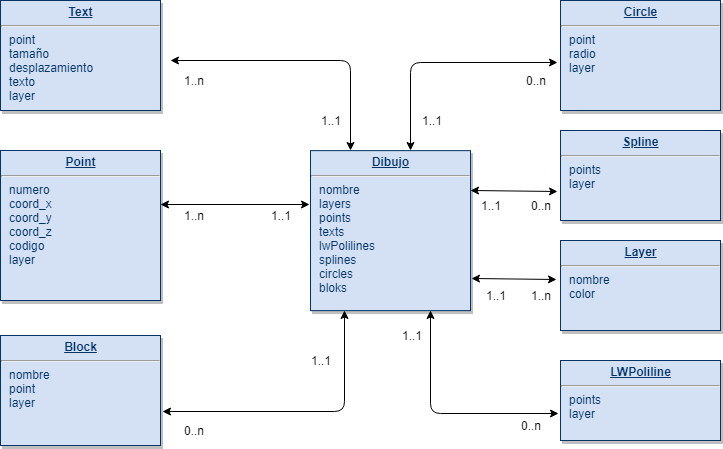
\includegraphics[width=0.9\textwidth]{DR-1}
	\caption{Diagrama relacional principal.}
	\label{fig:DR-1}
\end{figure}

En la Figura~\ref{fig:DR-2}, se ven las relaciones entre sí, del resto de elementos.

\begin{figure}[H]
	\centering
	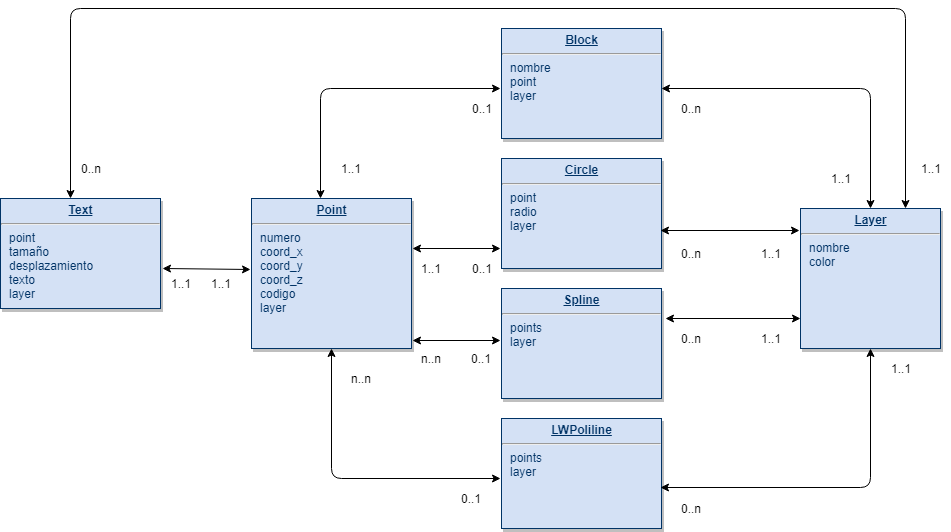
\includegraphics[width=1\textwidth]{DR-2}
	\caption{Diagrama relacional elementos del dibujo.}
	\label{fig:DR-2}
\end{figure}

\section{Diseño arquitectónico}

Como se ha detallado en la memoria (ver apartado 4.2. Patrones de diseño), para el diseño de la aplicación se ha utilizado el patrón arquitectónico \textbf{MTV}, que es similar al MCV, pero con alguna diferencia. \textbf{T} significa \emph{Template}, plantilla , que son los datos que se presentan al usuario y \textbf{V}significa vista, la capa de la lógica de negocios.
\textbf{MTV} es la arquitectura usada por \texttt{Flask}. 

%\imagen{MTV}{Esquema de un patrón MTV}
\begin{figure}[H]
	\centering
	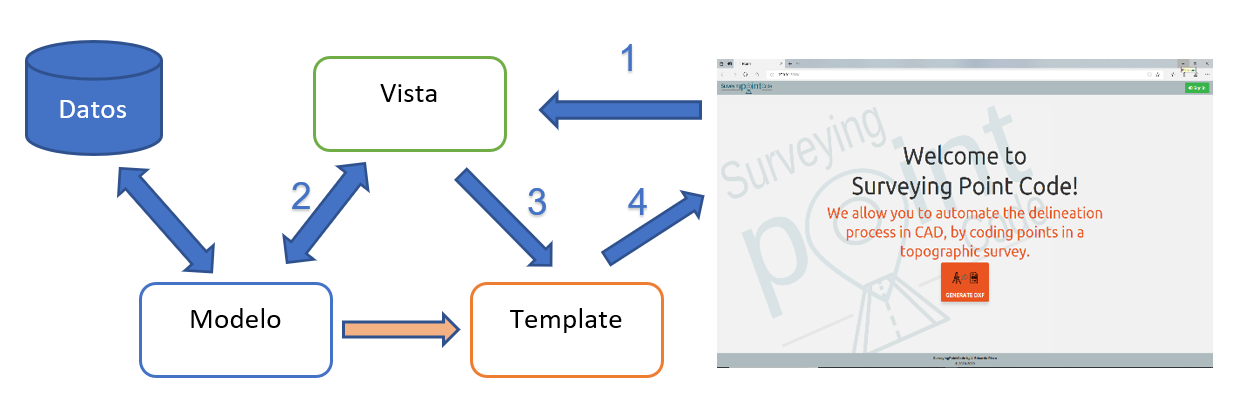
\includegraphics[width=0.5\textwidth]{MTV}
	\caption{Esquema de un patrón MTV.}
	\label{fig:MTV}
\end{figure}
Como sistema de base de datos se ha utilizado \textbf{PostGIS}. Para tener más independencia de la base de datos se ha optado por usar un \textbf{ORM}, \emph{SQLALchemy}. El uso de un ORM, nos simplificará el desarrollo si en un futuro se decide cambiar de base de datos.


\begin{figure}[H]
	\centering
	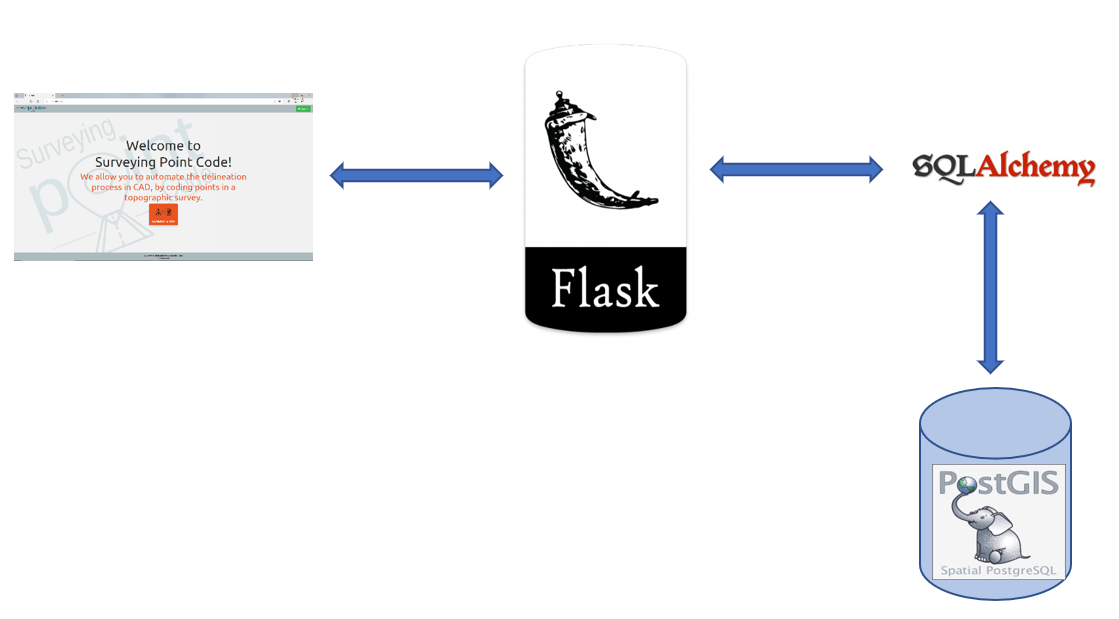
\includegraphics[width=0.5\textwidth]{Arq_1}
	\caption{Diseño arquitectónico con ORM y BBDD.}
	\label{fig:Arq_1}
\end{figure}

La aplicación se ha terminado de construir utilizando el sistema de contenedores \emph{Docker}. Con el uso de esta infraestructura se mejora la capacidad de ejecutar varios procesos y aplicaciones por separado y, al mismo tiempo, también conserva la seguridad que tendría con sistemas separados. Los contenedores \emph{Docker} son una especie de máquinas virtuales, pero más ligeras, que permiten  encapsular cualquier arquitectura, convirtiéndola en un contenedor portable y autosuficiente. 


\begin{figure}[H]
	\centering
	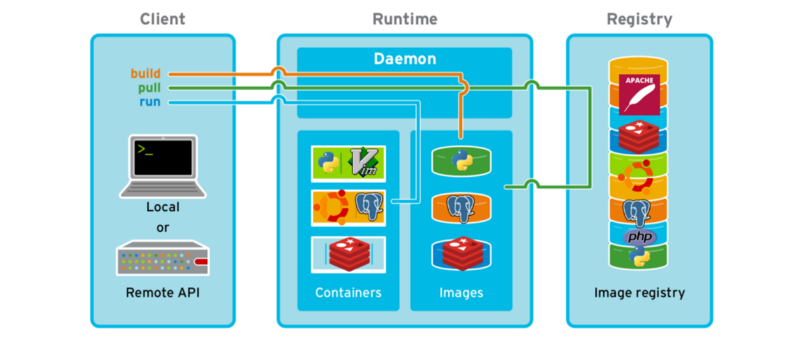
\includegraphics[width=0.7\textwidth]{Arq_docker}
	\caption{Arquitectura de \emph{Docker}\cite{arq_dock}.}
	\label{fig:Arq_docker}
\end{figure}

como se puede ver en la imagen anterior, \emph{Docker} está compuesto por tres partes:

\begin{itemize}
\item \emph{Docker client}: herramienta en línea de comandos, responsable para comunicarnos con el servidor \emph{Docker}. La comunicación se lleva a cabo mediante una \emph{RESTful API} a la cual solicitamos operaciones.

\item \emph{Docker Runtime}: este servicio, que se ejecuta como un demonio en un sistema operativo, construye, ejecuta y descarga las imágenes de los contenedores. El demonio puede ejecutarse en el mismo sistema que el cliente \emph{Docker} o de forma remota.

\item \emph{Docker Registry}: aquí se almacenan imágenes para uso público o privado. El conocido registro público es \emph{Docker Hub}, y almacena múltiples imágenes desarrolladas por la comunidad. Existe también la posibilidad de crear registros privados.

\end{itemize}

La arquitectura final basada en \emph{Docker} que se ha implementado, queda de la siguiente forma:

\begin{itemize}

\item \textbf{\emph{API Flask}}: contiene la aplicación desarrollada en \emph{Flask} y esta conectado con el contendedor \emph{PostGIS}.

\item \textbf{\emph{PostGIS}}: contiene la base de datos y esta conectado con los contendedores \emph{API Flask} y \emph{PgAdmin}.

\item \textbf{\emph{PgAdmin}}: contiene la aplicación \emph{PgAdmin 4}, para la gestión de la base de datos y esta conectado con el contendedor \emph{PostGIS}.
\end{itemize}

\begin{figure}[H]
	\centering
	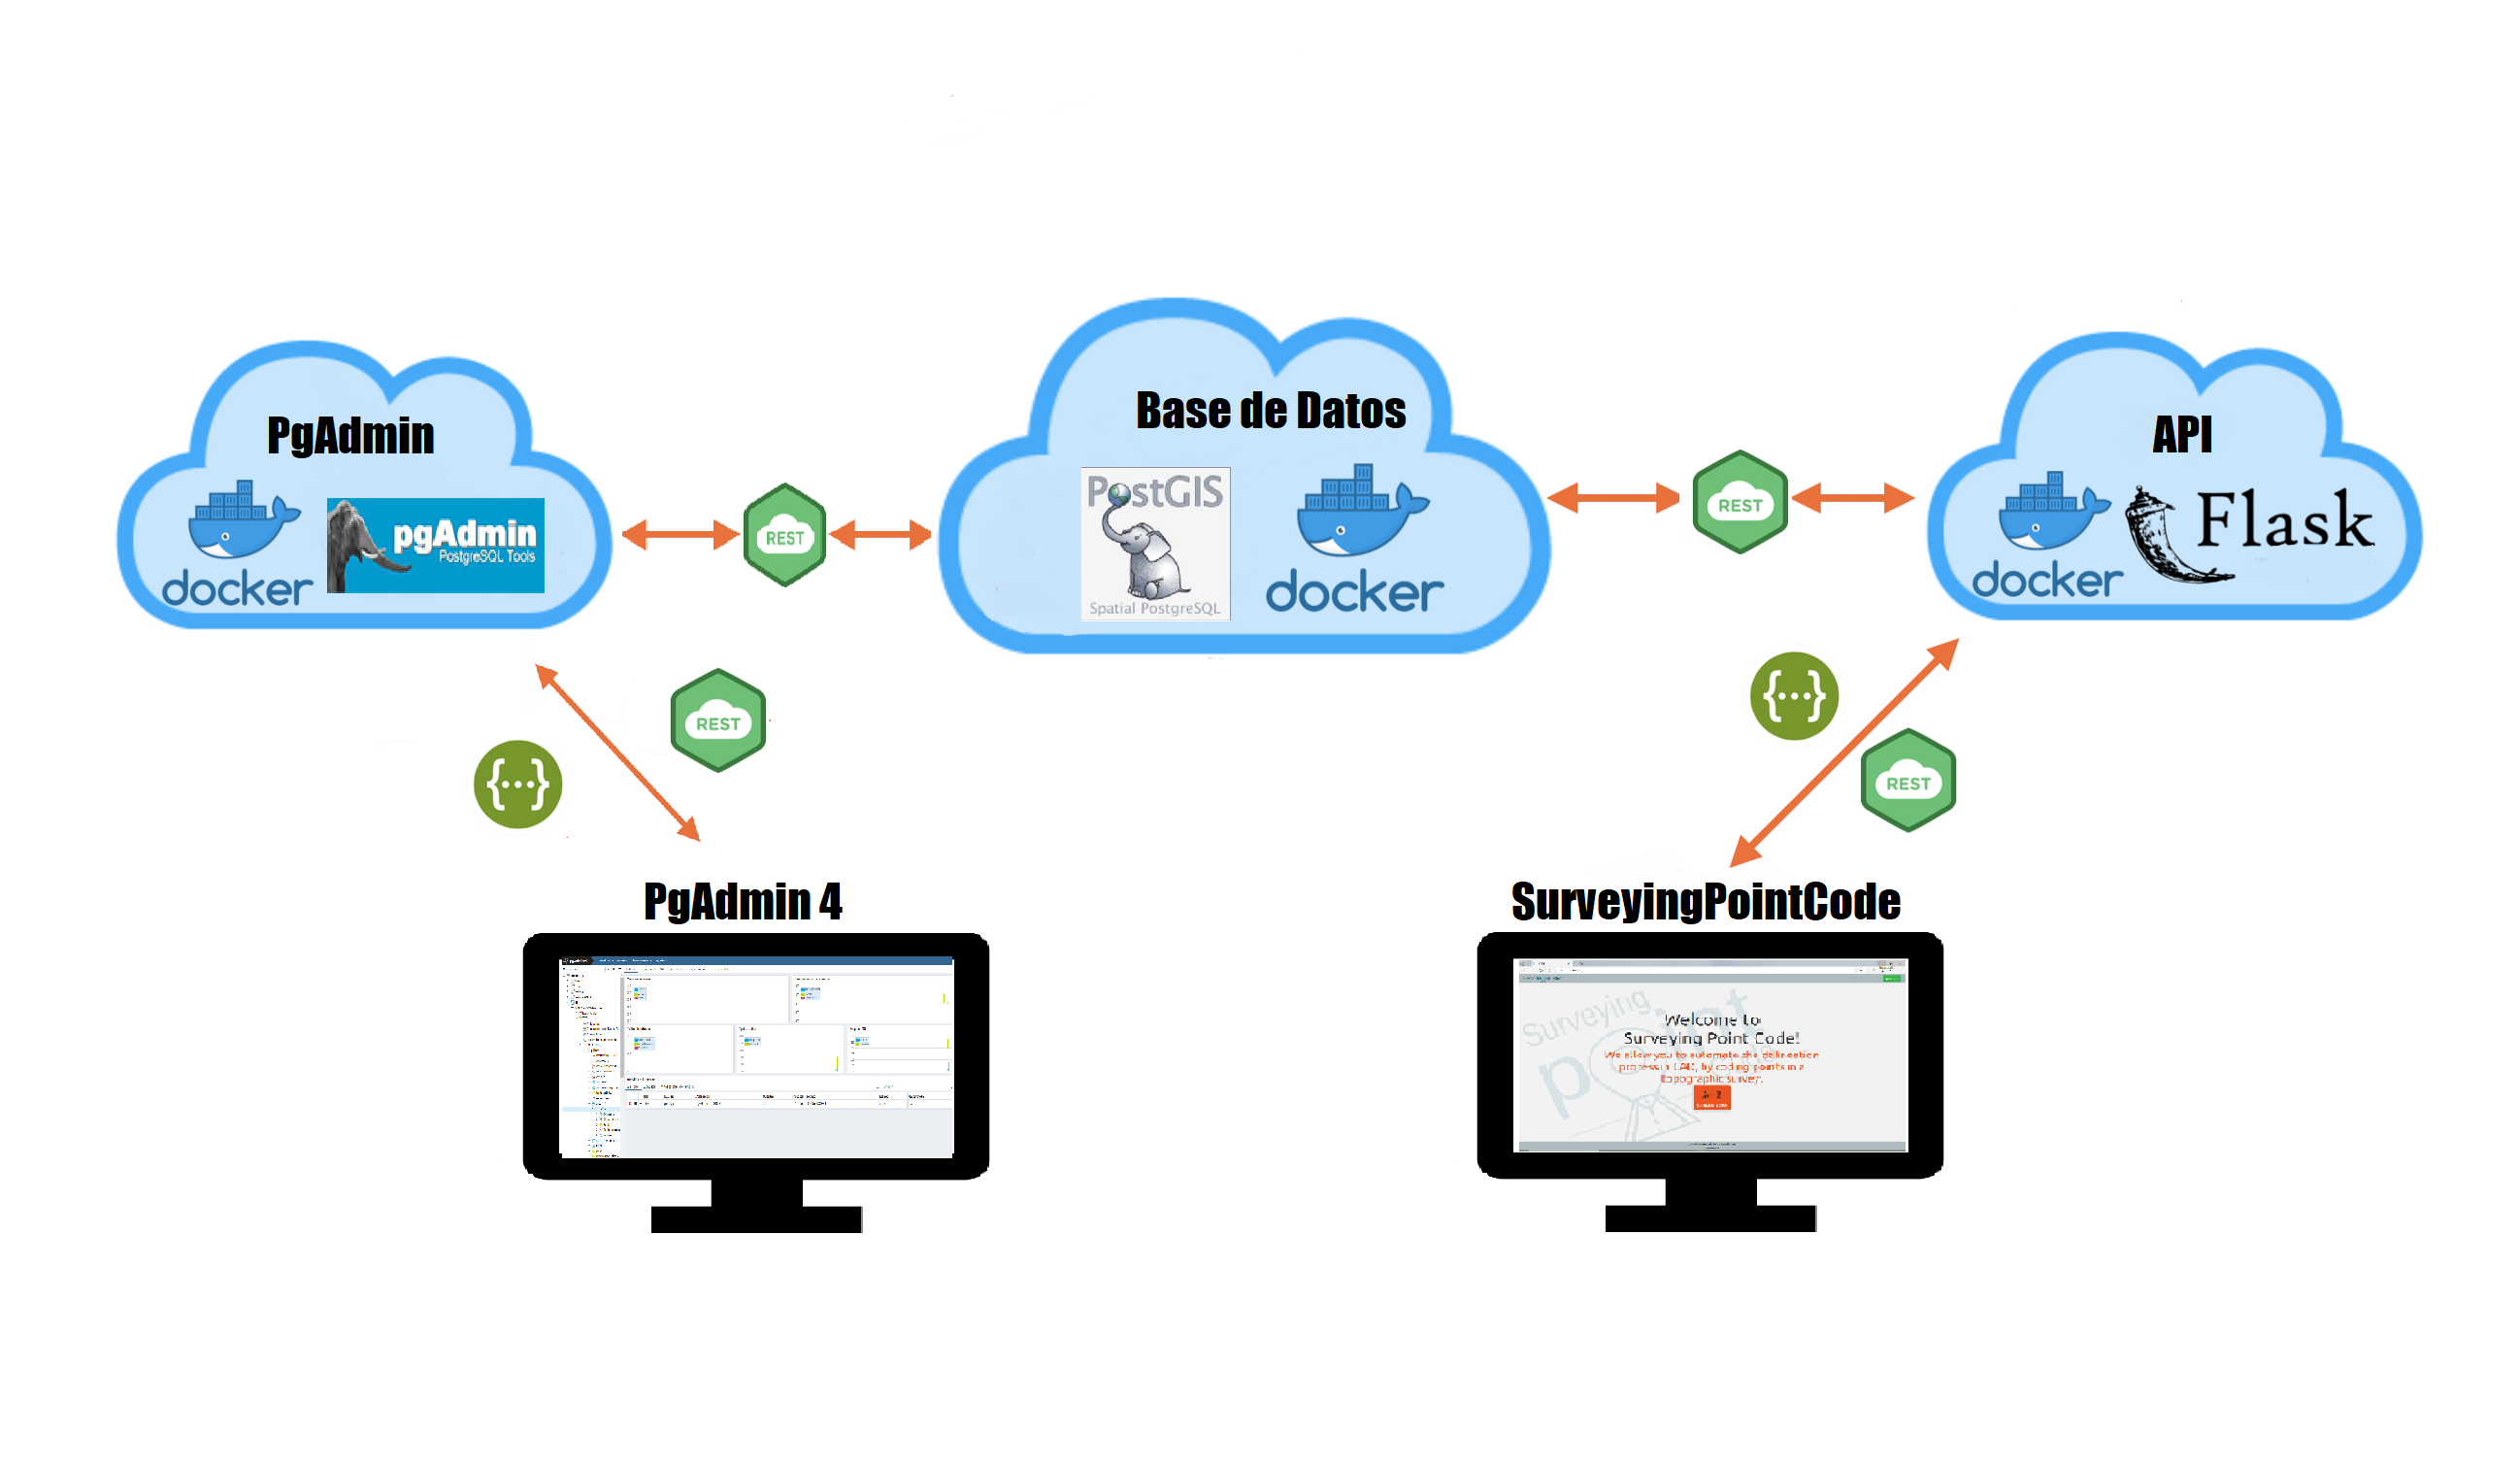
\includegraphics[width=1\textwidth]{Arq_SPC}
	\caption{Arquitectura final de la aplicación con \emph{Docker}}.
	\label{fig:Arq_SPC}
\end{figure}

\section{Diseño procedimental}










\apendice{Documentación técnica de programación}

\section{Introducción}
En este apartado se detalla la documentación técnica de programación, estructura de la aplicación, instalación de la aplicación, test realizados, etc. Datos necesarios que pueden servir de guía a cualquier programador pretenda continuar con este proyecto.

\section{Estructura de directorios}

\emph{Flask} permite una gran libertad a la hora de estructurar un proyecto, aunque por convención sigue una estructura determinada. Esta aplicación ha seguido esa estructura. A continuación se expone:

\begin{itemize}

\item \texttt{\textbf{SurveyingPointCode/:}} directorio raíz de la aplicación que contiene archivos como: \texttt{surveyingpointcode.py} y \texttt{config.py}, que son de inicio y configuración de la aplicación, respectivamente. También se encuentra un archivo con los requerimientos necesarios \texttt{requirements.txt} y un archivo con las variables de entorno que se deben cargar al sistema \texttt{app-env}. Por otra parte, se incluyen los archivos necesarios para el despliegue con \emph{Docker}, estos de detallarán más adelante.

\item \texttt{\textbf{SurveyingPointCode/app/:}} contiene todos los archivos que definen la lógica del negocio. 

\item \texttt{\textbf{SurveyingPointCode/app/templates/:}} contiene todos los archivos con las plantillas \emph{ html}. 

\item \texttt{\textbf{SurveyingPointCode/app/static/:}} contiene todos los archivos estáticos.

\item \texttt{\textbf{SurveyingPointCode/app/static/css:}} contiene todos los archivos con los estilos.

\item \texttt{\textbf{SurveyingPointCode/app/static/js:}} contiene todos los archivos \emph{JavaScript}.

\item \texttt{\textbf{SurveyingPointCode/app/static/images/:}} contiene todos los archivos con las imágenes de la que se usan en la aplicación Web.

\item \texttt{\textbf{SurveyingPointCode/app/static/webfonts/:}} contiene todos los archivos con las fuentes de la que se usan en la aplicación Web.

\item \texttt{\textbf{SurveyingPointCode/tmp/:}} contiene todos los archivos temporales que se generan en cada sesión, tanto los archivos subidos por el usuario, como las conversiones.

\item \texttt{\textbf{Archivos\_Prueba/:}} contiene diferentes archivos de ejemplo para cargar en la aplicación, tanto válidos como con errores.

\item \texttt{\textbf{Archivos\_Prueba/Datos\_de\_campo/:}} contiene diferentes archivos de campo, procedentes de un levantamiento topográfico.

\item \texttt{\textbf{Archivos\_Prueba/Configuración\_usuario/:}} contiene diferentes archivos de configuración de la conversión.

\item \texttt{\textbf{Archivos\_Prueba/Simbolos/:}} contiene diferentes archivos DXF, algunos válidos con símbolos definidos y otros vacíos.

\item \texttt{\textbf{Test\_unitarios/:}} contiene diferentes archivos para realizar los test unitarios.

\end{itemize}


\section{Manual del programador}

Este manual tiene como objetivo servir de referencia a futuros programadores que trabajen en la aplicación o a cualquier persona interesada en su construcción. 

Existen dos vías a seguir:

\begin{enumerate}

\item Configuración del entorno de desarrollo en un equipo instalando todas las herramientas necesarias. 

\item Utilizar \emph{Docker} como entorno de desarrollo. 

\end{enumerate}

En este proyecto se han seguido las dos vías. Se llevó a cabo todo el proceso con la primera, hasta que la aplicación estuvo montada completamente en \emph{Docker}, por lo que se siguió con la segunda vía. 
El proyecto se ha desarrollado utilizando un equipo con sistema operativo \emph{Linux} en su distribución \emph{Linux Mint 18.3 Sylvia}. Los comandos a continuación detallados son para ese sistema operativo.

\subsection{Configuración del entorno de desarrollo en un equipo}

Esta es la forma más convencional de realizar un desarrollo, instalar  las herramientas, bibliotecas y módulos en el equipo. A continuación se describen brevemente los pasos seguidos:

\begin{enumerate}

\item En primer lugar descargar el código de la aplicación que se encuentra en \emph{GitHub} o clonar el repositorio al equipo local.

\item Instalación de \emph{Anaconda} con Python 3.6. La opción de usar \emph{Anaconda} es para facilitar la opción de trabajar con entornos virtuales personalizados, sin necesidad de instalar dependencias directamente en nuestro equipo.

\item Creación de un entorno virtual en \emph{Anaconda}.

\texttt{conda create -n nombre\_de\_entorno python=3.6 anaconda}

\item Activar el entorno virtual en \emph{Anaconda}.

\texttt{source activate  nombre\_de\_entorno}

\item Instalar las dependencias dentro del entorno virtual creado. Para ello necesitamos el archivo \texttt{requirements.txt}, mencionado anteriormente.
\texttt{pip install -r requirements.txt}

\texttt Para trabajar con la base de datos \emph{PostGIS}, se utiliza un contenedor \emph{Docker}. En este punto se debe tener instalado \emph{Docker}. El contenedor de \emph{PostGIS} se crea con este comando:

\begin{verbatim}
sudo docker run --name=postgis --hostname=postgres --network=pgnetwork
-d -e POSTGRES_USER=tfg -e POSTGRES_PASS=f04f1b4d7734f0dc3c4da46f19c0a9f49b56
-e POSTGRES_DBNAME=tfg -e ALLOW_IP_RANGE=0.0.0.0/0 
-p 5432:5432 -v pg_data:/var/lib/postgresql --restart=always mdillon/postgis
\end{verbatim}

siendo sus parámetros de conexión con la BBDD:

\begin{verbatim}
user=tfg
password=f04f1b4d7734f0dc3c4da46f19c0a9f49b56
db_name=tfg
port=5432
host=postgis

\end{verbatim}


\end{enumerate}
El entorno de desarrollo está configurado. El \emph{IDE} o editor de texto utilizado es una opción personal del desarrollador, en este proyecto se ha usado \emph{PyCharm}.



\subsection{Utilizar \emph{Docker} como entorno de desarrollo.}

Entre las múltiples ventajas de usar \emph{Docker}, es importante destacar que se puede usar tanto en la etapa de desarrollo como, finalmente en el despliegue. Garantiza que el entorno de desarrollo va a ser siempre el mismo, independientemente del equipo en que se trabaje.

En este proyecto, el uso de \emph{Docker} facilitará la continuidad del desarrollo, solamente hace falta tener instalado en el equipo, la aplicación \emph{Docker}. Siguiendo las instrucciones del archivo \texttt{README.txt} que a continuación se enumeran:

\begin{enumerate}
\item Instalación de \emph{Docker.}
\item Instalación de \emph{Docker Compose.}
\item Clonar el repositorio.
\item Ejecutar en el directorio \texttt{SurveyingPointCode/}:

\texttt{sh app\_install.sh}

Cada vez que realicemos un cambio en el código, debemos actualizar este cambio en el contenedor correspondiente, y lo haremos de la siguiente forma:
\begin{enumerate}

\item Ejecutamos \texttt{docker-compose down} para detener el contendedor.

\item Ejecutamos \texttt{docker-compose up -d} para volver a construir los contenedores y levantarlos.
\end{enumerate}

\end{enumerate}

Los archivos \texttt{Dockerfile} y \texttt{docker-compose.yml}, ya comentados en el documento de la memoria( ver apartado Despliegue de la aplicación — \emph{Docker Compose}.), son la base para la construcción de los contenedores y por consiguiente, de los servicios ofrecidos. 

Como contrapunto, se ha encontrado una desventaja al usar \emph{Docker} como entorno de desarrollo, el tiempo invertido en volver a construir el contenedor. A medida que el proyecto crece y se van aumentando las dependencias, el tiempo de creación del contenedor se alarga. Es conveniente seguir investigando sobre como solucionar este problema.

\section{Compilación, instalación y ejecución del proyecto}\label{sec:instalacion}

Como en el apartado anterior la instalación de la aplicación es sencillo gracias al uso de \emph{Docker} y tambien garantiza que se va a comportar igual independientemente del equipo donde se instale. Siguiendo las instrucciones del archivo \texttt{README.txt} que a continuación se enumeran, se realiza la instalación:

\begin{enumerate}
\item Instalación de \emph{Docker.}
\item Instalación de \emph{Docker Compose.}
\item Clonar el repositorio.
\item Ejecutar en el directorio \texttt{SurveyingPointCode/}:

\begin{itemize}
\item Si se desea solo instalar a aplicación \emph{SurveyingPointCode}:

\texttt{sh app\_install.sh}

\item Si se desea instalar ademas la aplicación \emph{PgAdmin4}:

\texttt{sh app\_install\_pgadmin.sh}

\end{itemize}

\item Acceder en el navegador a la dirección \url{http://0.0.0.0:5000} para \emph{SurveyingPointCode}:

\item Acceder en el navegador a la dirección \url{http://0.0.0.0:80} para \emph{PgAdmin 4}:

\end{enumerate}


\section{Pruebas del sistema}

Para comprobar el funcionamiento de las funciones principales de la aplicación se han realizado una serie de test unitarios. 

Se ha utilizado la biblioteca de python \texttt{unittest}.

\newpage
\subsection{Caso de prueba CP-01}

\textbf{Descripción:} Comprueba si el número de capas creadas en un modelo de dibujo es correcto una vez cargado y procesado un archivo de campo, con la función \texttt{create\_layers()}.

\textbf{Datos de entrada:} \texttt{Example\_topographic\_1.txt}


\begin{longtable}[]{@{}llll@{}}
\toprule
\begin{minipage}[b]{0.6\columnwidth}\raggedright\strut
Función\strut
\end{minipage} & \begin{minipage}[b]{0.20\columnwidth}\raggedright\strut
Condición\strut
\end{minipage} & \begin{minipage}[b]{0.15\columnwidth}\raggedright\strut
Salida Esperada\strut
\end{minipage} & \begin{minipage}[b]{0.05\columnwidth}\raggedright\strut
Ok\strut
\end{minipage}\tabularnewline
\midrule
\endhead
\begin{minipage}[t]{0.6\columnwidth}\raggedright\strut
test\_create\_layers\_number()\strut
\end{minipage} & \begin{minipage}[t]{0.20\columnwidth}\raggedright\strut
¿Es igual?\strut
\end{minipage} & \begin{minipage}[t]{0.15\columnwidth}\raggedright\strut
8\strut
\end{minipage} & \begin{minipage}[t]{0.05\columnwidth}\raggedright\strut
Si\strut
\end{minipage}\tabularnewline
\begin{minipage}[t]{0.6\columnwidth}\raggedright\strut
\strut
\end{minipage} & \begin{minipage}[t]{0.20\columnwidth}\raggedright\strut
¿No es igual?\strut
\end{minipage} & \begin{minipage}[t]{0.15\columnwidth}\raggedright\strut
0\strut
\end{minipage} & \begin{minipage}[t]{0.05\columnwidth}\raggedright\strut
Si\strut
\end{minipage}\tabularnewline

\bottomrule
\caption{Caso de prueba CP-01.}
\end{longtable}

\subsection{Caso de prueba CP-02}

\textbf{Descripción:} Comprueba el nombre de las capas creadas es correcto una vez cargado y procesado un archivo de campo, con la función \texttt{create\_layers()}.

\textbf{Datos de entrada:} \texttt{Example\_topographic\_1.txt}


\begin{longtable}[]{@{}llll@{}}
\toprule
\begin{minipage}[b]{0.6\columnwidth}\raggedright\strut
Función\strut
\end{minipage} & \begin{minipage}[b]{0.20\columnwidth}\raggedright\strut
Condición\strut
\end{minipage} & \begin{minipage}[b]{0.15\columnwidth}\raggedright\strut
Salida Esperada\strut
\end{minipage} & \begin{minipage}[b]{0.05\columnwidth}\raggedright\strut
Ok\strut
\end{minipage}\tabularnewline
\midrule
\endhead
\begin{minipage}[t]{0.6\columnwidth}\raggedright\strut
test\_create\_layers\_types()\strut
\end{minipage} & \begin{minipage}[t]{0.20\columnwidth}\raggedright\strut
¿Contiene?\strut
\end{minipage} & \begin{minipage}[t]{0.15\columnwidth}\raggedright\strut
Si\strut
\end{minipage} & \begin{minipage}[t]{0.05\columnwidth}\raggedright\strut
Si\strut
\end{minipage}\tabularnewline
\bottomrule
\caption{Caso de prueba CP-02.}
\end{longtable}

\subsection{Caso de prueba CP-03}

\textbf{Descripción:} Comprueba si el número de puntos insertados en un modelo de dibujo es correcto una vez cargado y procesado un archivo de campo, con la función \texttt{get\_points()}.

\textbf{Datos de entrada:} \texttt{Example\_topographic\_1.txt}


\begin{longtable}[]{@{}llll@{}}
\toprule
\begin{minipage}[b]{0.6\columnwidth}\raggedright\strut
Función\strut
\end{minipage} & \begin{minipage}[b]{0.20\columnwidth}\raggedright\strut
Condición\strut
\end{minipage} & \begin{minipage}[b]{0.15\columnwidth}\raggedright\strut
Salida Esperada\strut
\end{minipage} & \begin{minipage}[b]{0.05\columnwidth}\raggedright\strut
Ok\strut
\end{minipage}\tabularnewline
\midrule
\endhead
\begin{minipage}[t]{0.6\columnwidth}\raggedright\strut
test\_create\_points\_number\_file\_correct()\strut
\end{minipage} & \begin{minipage}[t]{0.20\columnwidth}\raggedright\strut
¿Es igual?\strut
\end{minipage} & \begin{minipage}[t]{0.15\columnwidth}\raggedright\strut
42\strut
\end{minipage} & \begin{minipage}[t]{0.05\columnwidth}\raggedright\strut
Si\strut
\end{minipage}\tabularnewline
\begin{minipage}[t]{0.6\columnwidth}\raggedright\strut
\strut
\end{minipage} & \begin{minipage}[t]{0.20\columnwidth}\raggedright\strut
¿No es igual?\strut
\end{minipage} & \begin{minipage}[t]{0.15\columnwidth}\raggedright\strut
0\strut
\end{minipage} & \begin{minipage}[t]{0.05\columnwidth}\raggedright\strut
Si\strut
\end{minipage}\tabularnewline

\bottomrule
\caption{Caso de prueba CP-03.}
\end{longtable}

\subsection{Caso de prueba CP-04}

\textbf{Descripción:} Comprueba si el número de textos insertados en un modelo de dibujo es correcto una vez cargado y procesado un archivo de campo, con la función \texttt{get\_points()}.

\textbf{Datos de entrada:} \texttt{Example\_topographic\_1.txt}


\begin{longtable}[]{@{}llll@{}}
\toprule
\begin{minipage}[b]{0.6\columnwidth}\raggedright\strut
Función\strut
\end{minipage} & \begin{minipage}[b]{0.20\columnwidth}\raggedright\strut
Condición\strut
\end{minipage} & \begin{minipage}[b]{0.15\columnwidth}\raggedright\strut
Salida Esperada\strut
\end{minipage} & \begin{minipage}[b]{0.05\columnwidth}\raggedright\strut
Ok\strut
\end{minipage}\tabularnewline
\midrule
\endhead
\begin{minipage}[t]{0.6\columnwidth}\raggedright\strut
test\_create\_points\_texts\_file\_correct()\strut
\end{minipage} & \begin{minipage}[t]{0.20\columnwidth}\raggedright\strut
¿Es igual?\strut
\end{minipage} & \begin{minipage}[t]{0.15\columnwidth}\raggedright\strut
126\strut
\end{minipage} & \begin{minipage}[t]{0.05\columnwidth}\raggedright\strut
Si\strut
\end{minipage}\tabularnewline
\begin{minipage}[t]{0.6\columnwidth}\raggedright\strut
\strut
\end{minipage} & \begin{minipage}[t]{0.20\columnwidth}\raggedright\strut
¿No es igual?\strut
\end{minipage} & \begin{minipage}[t]{0.15\columnwidth}\raggedright\strut
0\strut
\end{minipage} & \begin{minipage}[t]{0.05\columnwidth}\raggedright\strut
Si\strut
\end{minipage}\tabularnewline

\bottomrule
\caption{Caso de prueba CP-04.}
\end{longtable}

\subsection{Caso de prueba CP-05}

\textbf{Descripción:} Comprueba si el número de círculos insertados en un modelo de dibujo es correcto una vez cargado y procesado un archivo de campo, con la función \texttt{get\_circles()}.

\textbf{Datos de entrada:} \texttt{Example\_topographic\_1.txt}


\begin{longtable}[]{@{}llll@{}}
\toprule
\begin{minipage}[b]{0.6\columnwidth}\raggedright\strut
Función\strut
\end{minipage} & \begin{minipage}[b]{0.20\columnwidth}\raggedright\strut
Condición\strut
\end{minipage} & \begin{minipage}[b]{0.15\columnwidth}\raggedright\strut
Salida Esperada\strut
\end{minipage} & \begin{minipage}[b]{0.05\columnwidth}\raggedright\strut
Ok\strut
\end{minipage}\tabularnewline
\midrule
\endhead
\begin{minipage}[t]{0.6\columnwidth}\raggedright\strut
test\_create\_circles\_number()\strut
\end{minipage} & \begin{minipage}[t]{0.20\columnwidth}\raggedright\strut
¿Es igual?\strut
\end{minipage} & \begin{minipage}[t]{0.15\columnwidth}\raggedright\strut
2\strut
\end{minipage} & \begin{minipage}[t]{0.05\columnwidth}\raggedright\strut
Si\strut
\end{minipage}\tabularnewline
\begin{minipage}[t]{0.6\columnwidth}\raggedright\strut
\strut
\end{minipage} & \begin{minipage}[t]{0.20\columnwidth}\raggedright\strut
¿No es igual?\strut
\end{minipage} & \begin{minipage}[t]{0.15\columnwidth}\raggedright\strut
0\strut
\end{minipage} & \begin{minipage}[t]{0.05\columnwidth}\raggedright\strut
Si\strut
\end{minipage}\tabularnewline

\bottomrule
\caption{Caso de prueba CP-05.}
\end{longtable}

\subsection{Caso de prueba CP-06}

\textbf{Descripción:} Comprueba si el número de \emph{splines} insertados en un modelo de dibujo es correcto una vez cargado y procesado un archivo de campo, con la función \texttt{get\_splines()}.

\textbf{Datos de entrada:} \texttt{Example\_topographic\_1.txt}


\begin{longtable}[]{@{}llll@{}}
\toprule
\begin{minipage}[b]{0.6\columnwidth}\raggedright\strut
Función\strut
\end{minipage} & \begin{minipage}[b]{0.20\columnwidth}\raggedright\strut
Condición\strut
\end{minipage} & \begin{minipage}[b]{0.15\columnwidth}\raggedright\strut
Salida Esperada\strut
\end{minipage} & \begin{minipage}[b]{0.05\columnwidth}\raggedright\strut
Ok\strut
\end{minipage}\tabularnewline
\midrule
\endhead
\begin{minipage}[t]{0.6\columnwidth}\raggedright\strut
test\_create\_splines\_number()\strut
\end{minipage} & \begin{minipage}[t]{0.20\columnwidth}\raggedright\strut
¿Es igual?\strut
\end{minipage} & \begin{minipage}[t]{0.15\columnwidth}\raggedright\strut
1\strut
\end{minipage} & \begin{minipage}[t]{0.05\columnwidth}\raggedright\strut
Si\strut
\end{minipage}\tabularnewline
\begin{minipage}[t]{0.6\columnwidth}\raggedright\strut
\strut
\end{minipage} & \begin{minipage}[t]{0.20\columnwidth}\raggedright\strut
¿No es igual?\strut
\end{minipage} & \begin{minipage}[t]{0.15\columnwidth}\raggedright\strut
0\strut
\end{minipage} & \begin{minipage}[t]{0.05\columnwidth}\raggedright\strut
Si\strut
\end{minipage}\tabularnewline

\bottomrule
\caption{Caso de prueba CP-06.}
\end{longtable}

\subsection{Caso de prueba CP-07}

\textbf{Descripción:} Comprueba si el número de líneas insertadas en un modelo de dibujo es correcto una vez cargado y procesado un archivo de campo, con la función \texttt{get\_lines()}.

\textbf{Datos de entrada:} \texttt{Example\_topographic\_1.txt}


\begin{longtable}[]{@{}llll@{}}
\toprule
\begin{minipage}[b]{0.6\columnwidth}\raggedright\strut
Función\strut
\end{minipage} & \begin{minipage}[b]{0.20\columnwidth}\raggedright\strut
Condición\strut
\end{minipage} & \begin{minipage}[b]{0.15\columnwidth}\raggedright\strut
Salida Esperada\strut
\end{minipage} & \begin{minipage}[b]{0.05\columnwidth}\raggedright\strut
Ok\strut
\end{minipage}\tabularnewline
\midrule
\endhead
\begin{minipage}[t]{0.6\columnwidth}\raggedright\strut
test\_create\_lines\_number()\strut
\end{minipage} & \begin{minipage}[t]{0.20\columnwidth}\raggedright\strut
¿Es igual?\strut
\end{minipage} & \begin{minipage}[t]{0.15\columnwidth}\raggedright\strut
5\strut
\end{minipage} & \begin{minipage}[t]{0.05\columnwidth}\raggedright\strut
Si\strut
\end{minipage}\tabularnewline
\begin{minipage}[t]{0.6\columnwidth}\raggedright\strut
\strut
\end{minipage} & \begin{minipage}[t]{0.20\columnwidth}\raggedright\strut
¿No es igual?\strut
\end{minipage} & \begin{minipage}[t]{0.15\columnwidth}\raggedright\strut
0\strut
\end{minipage} & \begin{minipage}[t]{0.05\columnwidth}\raggedright\strut
Si\strut
\end{minipage}\tabularnewline

\bottomrule
\caption{Caso de prueba CP-07.}
\end{longtable}

\subsection{Caso de prueba CP-08}

\textbf{Descripción:} Comprueba si el número de cuadrados insertados en un modelo de dibujo es correcto una vez cargado y procesado un archivo de campo, con la función \texttt{get\_squares()}.

\textbf{Datos de entrada:} \texttt{Example\_topographic\_1.txt}


\begin{longtable}[]{@{}llll@{}}
\toprule
\begin{minipage}[b]{0.6\columnwidth}\raggedright\strut
Función\strut
\end{minipage} & \begin{minipage}[b]{0.20\columnwidth}\raggedright\strut
Condición\strut
\end{minipage} & \begin{minipage}[b]{0.15\columnwidth}\raggedright\strut
Salida Esperada\strut
\end{minipage} & \begin{minipage}[b]{0.05\columnwidth}\raggedright\strut
Ok\strut
\end{minipage}\tabularnewline
\midrule
\endhead
\begin{minipage}[t]{0.6\columnwidth}\raggedright\strut
test\_create\_squares\_number()\strut
\end{minipage} & \begin{minipage}[t]{0.20\columnwidth}\raggedright\strut
¿Es igual?\strut
\end{minipage} & \begin{minipage}[t]{0.15\columnwidth}\raggedright\strut
5\strut
\end{minipage} & \begin{minipage}[t]{0.05\columnwidth}\raggedright\strut
Si\strut
\end{minipage}\tabularnewline
\begin{minipage}[t]{0.6\columnwidth}\raggedright\strut
\strut
\end{minipage} & \begin{minipage}[t]{0.20\columnwidth}\raggedright\strut
¿No es igual?\strut
\end{minipage} & \begin{minipage}[t]{0.15\columnwidth}\raggedright\strut
0\strut
\end{minipage} & \begin{minipage}[t]{0.05\columnwidth}\raggedright\strut
Si\strut
\end{minipage}\tabularnewline

\bottomrule
\caption{Caso de prueba CP-08.}
\end{longtable}

\subsection{Caso de prueba CP-09}

\textbf{Descripción:} Comprueba si el número de rectángulos insertados en un modelo de dibujo es correcto una vez cargado y procesado un archivo de campo, con la función \texttt{get\_rectangles()}.

\textbf{Datos de entrada:} \texttt{Example\_topographic\_1.txt}


\begin{longtable}[]{@{}llll@{}}
\toprule
\begin{minipage}[b]{0.6\columnwidth}\raggedright\strut
Función\strut
\end{minipage} & \begin{minipage}[b]{0.20\columnwidth}\raggedright\strut
Condición\strut
\end{minipage} & \begin{minipage}[b]{0.15\columnwidth}\raggedright\strut
Salida Esperada\strut
\end{minipage} & \begin{minipage}[b]{0.05\columnwidth}\raggedright\strut
Ok\strut
\end{minipage}\tabularnewline
\midrule
\endhead
\begin{minipage}[t]{0.6\columnwidth}\raggedright\strut
test\_create\_squares\_number()\strut
\end{minipage} & \begin{minipage}[t]{0.20\columnwidth}\raggedright\strut
¿Es igual?\strut
\end{minipage} & \begin{minipage}[t]{0.15\columnwidth}\raggedright\strut
1\strut
\end{minipage} & \begin{minipage}[t]{0.05\columnwidth}\raggedright\strut
Si\strut
\end{minipage}\tabularnewline
\begin{minipage}[t]{0.6\columnwidth}\raggedright\strut
\strut
\end{minipage} & \begin{minipage}[t]{0.20\columnwidth}\raggedright\strut
¿No es igual?\strut
\end{minipage} & \begin{minipage}[t]{0.15\columnwidth}\raggedright\strut
0\strut
\end{minipage} & \begin{minipage}[t]{0.05\columnwidth}\raggedright\strut
Si\strut
\end{minipage}\tabularnewline

\bottomrule
\caption{Caso de prueba CP-09.}
\end{longtable}

\subsection{Caso de prueba CP-10}

\textbf{Descripción:} Comprueba que un archivo sin círculos no crea ningún círculo en un modelo de dibujo una vez cargado y procesado un archivo de campo, con la función \texttt{get\_circles()}.

\textbf{Datos de entrada:} \texttt{Example\_topographic\_2.txt}


\begin{longtable}[]{@{}llll@{}}
\toprule
\begin{minipage}[b]{0.6\columnwidth}\raggedright\strut
Función\strut
\end{minipage} & \begin{minipage}[b]{0.20\columnwidth}\raggedright\strut
Condición\strut
\end{minipage} & \begin{minipage}[b]{0.15\columnwidth}\raggedright\strut
Salida Esperada\strut
\end{minipage} & \begin{minipage}[b]{0.05\columnwidth}\raggedright\strut
Ok\strut
\end{minipage}\tabularnewline
\midrule
\endhead
\begin{minipage}[t]{0.6\columnwidth}\raggedright\strut
test\_not\_create\_circles()\strut
\end{minipage} & \begin{minipage}[t]{0.20\columnwidth}\raggedright\strut
¿Es igual?\strut
\end{minipage} & \begin{minipage}[t]{0.15\columnwidth}\raggedright\strut
0\strut
\end{minipage} & \begin{minipage}[t]{0.05\columnwidth}\raggedright\strut
Si\strut
\end{minipage}\tabularnewline

\bottomrule
\caption{Caso de prueba CP-10.}
\end{longtable}

\subsection{Caso de prueba CP-11}

\textbf{Descripción:} Comprueba que un archivo sin \emph{splines} no crea ninguna \emph{spline} en un modelo de dibujo una vez cargado y procesado un archivo de campo, con la función \texttt{get\_splines()}.

\textbf{Datos de entrada:} \texttt{Example\_topographic\_2.txt}


\begin{longtable}[]{@{}llll@{}}
\toprule
\begin{minipage}[b]{0.6\columnwidth}\raggedright\strut
Función\strut
\end{minipage} & \begin{minipage}[b]{0.20\columnwidth}\raggedright\strut
Condición\strut
\end{minipage} & \begin{minipage}[b]{0.15\columnwidth}\raggedright\strut
Salida Esperada\strut
\end{minipage} & \begin{minipage}[b]{0.05\columnwidth}\raggedright\strut
Ok\strut
\end{minipage}\tabularnewline
\midrule
\endhead
\begin{minipage}[t]{0.6\columnwidth}\raggedright\strut
test\_not\_create\_splines()\strut
\end{minipage} & \begin{minipage}[t]{0.20\columnwidth}\raggedright\strut
¿Es igual?\strut
\end{minipage} & \begin{minipage}[t]{0.15\columnwidth}\raggedright\strut
0\strut
\end{minipage} & \begin{minipage}[t]{0.05\columnwidth}\raggedright\strut
Si\strut
\end{minipage}\tabularnewline

\bottomrule
\caption{Caso de prueba CP-11.}
\end{longtable}

\subsection{Caso de prueba CP-12}

\textbf{Descripción:} Comprueba que un archivo sin líneas no crea ninguna línea en un modelo de dibujo una vez cargado y procesado un archivo de campo, con la función \texttt{get\_lines()}.

\textbf{Datos de entrada:} \texttt{Example\_topographic\_2.txt}


\begin{longtable}[]{@{}llll@{}}
\toprule
\begin{minipage}[b]{0.6\columnwidth}\raggedright\strut
Función\strut
\end{minipage} & \begin{minipage}[b]{0.20\columnwidth}\raggedright\strut
Condición\strut
\end{minipage} & \begin{minipage}[b]{0.15\columnwidth}\raggedright\strut
Salida Esperada\strut
\end{minipage} & \begin{minipage}[b]{0.05\columnwidth}\raggedright\strut
Ok\strut
\end{minipage}\tabularnewline
\midrule
\endhead
\begin{minipage}[t]{0.6\columnwidth}\raggedright\strut
test\_not\_create\_lines()\strut
\end{minipage} & \begin{minipage}[t]{0.20\columnwidth}\raggedright\strut
¿Es igual?\strut
\end{minipage} & \begin{minipage}[t]{0.15\columnwidth}\raggedright\strut
0\strut
\end{minipage} & \begin{minipage}[t]{0.05\columnwidth}\raggedright\strut
Si\strut
\end{minipage}\tabularnewline

\bottomrule
\caption{Caso de prueba CP-12.}
\end{longtable}


\subsection{Caso de prueba CP-13}

\textbf{Descripción:} Comprueba que un archivo sin cuadrados ni rectángulos, no los crea en un modelo de dibujo una vez cargado y procesado un archivo de campo, con la función \texttt{get\_lines()}.

\textbf{Datos de entrada:} \texttt{Example\_topographic\_2.txt}


\begin{longtable}[]{@{}llll@{}}
\toprule
\begin{minipage}[b]{0.6\columnwidth}\raggedright\strut
Función\strut
\end{minipage} & \begin{minipage}[b]{0.20\columnwidth}\raggedright\strut
Condición\strut
\end{minipage} & \begin{minipage}[b]{0.15\columnwidth}\raggedright\strut
Salida Esperada\strut
\end{minipage} & \begin{minipage}[b]{0.05\columnwidth}\raggedright\strut
Ok\strut
\end{minipage}\tabularnewline
\midrule
\endhead
\begin{minipage}[t]{0.6\columnwidth}\raggedright\strut
test\_not\_create\_squares\_rectangles()\strut
\end{minipage} & \begin{minipage}[t]{0.20\columnwidth}\raggedright\strut
¿Es igual?\strut
\end{minipage} & \begin{minipage}[t]{0.15\columnwidth}\raggedright\strut
0\strut
\end{minipage} & \begin{minipage}[t]{0.05\columnwidth}\raggedright\strut
Si\strut
\end{minipage}\tabularnewline

\bottomrule
\caption{Caso de prueba CP-13.}
\end{longtable}

\subsection{Caso de prueba CP-14}

\textbf{Descripción:} Comprueba que use calculan correctamente el acimut y la distancia entre dos puntos, a y b, con la función \texttt{calculate\_azimut\_distance()}

\textbf{Datos de entrada:} \texttt{a = [1, (0, 0, 0), 'E'] y  b = [2, (100, 100, 0), 'E']}


\begin{longtable}[]{@{}llll@{}}
\toprule
\begin{minipage}[b]{0.6\columnwidth}\raggedright\strut
Función\strut
\end{minipage} & \begin{minipage}[b]{0.20\columnwidth}\raggedright\strut
Condición\strut
\end{minipage} & \begin{minipage}[b]{0.15\columnwidth}\raggedright\strut
Salida Esperada\strut
\end{minipage} & \begin{minipage}[b]{0.05\columnwidth}\raggedright\strut
Ok\strut
\end{minipage}\tabularnewline
\midrule
\endhead
\begin{minipage}[t]{0.6\columnwidth}\raggedright\strut
test\_azimut\_distance()\strut
\end{minipage} & \begin{minipage}[t]{0.20\columnwidth}\raggedright\strut
¿Es igual?\strut
\end{minipage} & \begin{minipage}[t]{0.15\columnwidth}\raggedright\strut
az=45º dist=141.4213\strut
\end{minipage} & \begin{minipage}[t]{0.05\columnwidth}\raggedright\strut
Si\strut
\end{minipage}\tabularnewline
\begin{minipage}[t]{0.6\columnwidth}\raggedright\strut
\strut
\end{minipage} & \begin{minipage}[t]{0.20\columnwidth}\raggedright\strut
¿No es igual?\strut
\end{minipage} & \begin{minipage}[t]{0.15\columnwidth}\raggedright\strut
az=50º dist=145\strut
\end{minipage} & \begin{minipage}[t]{0.05\columnwidth}\raggedright\strut
Si\strut
\end{minipage}\tabularnewline

\bottomrule
\caption{Caso de prueba CP-14.}
\end{longtable}



\subsection{Caso de prueba CP-15}

\textbf{Descripción:} Comprueba que se calculan correctamente el incremento de $X$ y de $Y$, entre dos puntos, conociendo el acimut y la distancia entre ellos, con la función \texttt{calculate\_increment\_x\_y()}

\textbf{Datos de entrada:} \texttt{az = 45º y dist = 141.4213562373095}
\newpage

\begin{longtable}[]{@{}llll@{}}
\toprule
\begin{minipage}[b]{0.6\columnwidth}\raggedright\strut
Función\strut
\end{minipage} & \begin{minipage}[b]{0.20\columnwidth}\raggedright\strut
Condición\strut
\end{minipage} & \begin{minipage}[b]{0.15\columnwidth}\raggedright\strut
Salida Esperada\strut
\end{minipage} & \begin{minipage}[b]{0.05\columnwidth}\raggedright\strut
Ok\strut
\end{minipage}\tabularnewline
\midrule
\endhead
\begin{minipage}[t]{0.6\columnwidth}\raggedright\strut
test\_increment\_x\_y()\strut
\end{minipage} & \begin{minipage}[t]{0.20\columnwidth}\raggedright\strut
¿Es igual?\strut
\end{minipage} & \begin{minipage}[t]{0.15\columnwidth}\raggedright\strut
In\_x=100 In\_y=100\strut
\end{minipage} & \begin{minipage}[t]{0.05\columnwidth}\raggedright\strut
Si\strut
\end{minipage}\tabularnewline
\begin{minipage}[t]{0.6\columnwidth}\raggedright\strut
\strut
\end{minipage} & \begin{minipage}[t]{0.20\columnwidth}\raggedright\strut
¿No es igual?\strut
\end{minipage} & \begin{minipage}[t]{0.15\columnwidth}\raggedright\strut
In\_x=150 In\_y=145\strut
\end{minipage} & \begin{minipage}[t]{0.05\columnwidth}\raggedright\strut
Si\strut
\end{minipage}\tabularnewline

\bottomrule
\caption{Caso de prueba CP-15.}
\end{longtable}


\subsection{Caso de prueba CP-16}

\textbf{Descripción:} Comprueba que se calculan correctamente un angulo, introduciendo un angulo y una distancia positiva o negativa, con la función \texttt{calculate\_angle()}

\textbf{Datos de entrada:} \texttt{az = 125º y dist =-10}


\begin{longtable}[]{@{}llll@{}}
\toprule
\begin{minipage}[b]{0.6\columnwidth}\raggedright\strut
Función\strut
\end{minipage} & \begin{minipage}[b]{0.20\columnwidth}\raggedright\strut
Condición\strut
\end{minipage} & \begin{minipage}[b]{0.15\columnwidth}\raggedright\strut
Salida Esperada\strut
\end{minipage} & \begin{minipage}[b]{0.05\columnwidth}\raggedright\strut
Ok\strut
\end{minipage}\tabularnewline
\midrule
\endhead
\begin{minipage}[t]{0.6\columnwidth}\raggedright\strut
test\_angle\_direction()\strut
\end{minipage} & \begin{minipage}[t]{0.20\columnwidth}\raggedright\strut
¿Es igual?\strut
\end{minipage} & \begin{minipage}[t]{0.15\columnwidth}\raggedright\strut
35º\strut
\end{minipage} & \begin{minipage}[t]{0.05\columnwidth}\raggedright\strut
Si\strut
\end{minipage}\tabularnewline
\begin{minipage}[t]{0.6\columnwidth}\raggedright\strut
\strut
\end{minipage} & \begin{minipage}[t]{0.20\columnwidth}\raggedright\strut
¿No es igual?\strut
\end{minipage} & \begin{minipage}[t]{0.15\columnwidth}\raggedright\strut
215º\strut
\end{minipage} & \begin{minipage}[t]{0.05\columnwidth}\raggedright\strut
Si\strut
\end{minipage}\tabularnewline

\bottomrule
\caption{Caso de prueba CP-16.}
\end{longtable}

\subsection{Caso de prueba CP-17}

\textbf{Descripción:} Comprueba si se extraen correctamente los símbolos de un archivo DXF subido por el usuario y también comprueba que se han extraído todos, con la función  \texttt{upload\_symbols\_file()}

\textbf{Datos de entrada:} \texttt{Example\_simbology.dxf}


\begin{longtable}[]{@{}llll@{}}
\toprule
\begin{minipage}[b]{0.6\columnwidth}\raggedright\strut
Función\strut
\end{minipage} & \begin{minipage}[b]{0.20\columnwidth}\raggedright\strut
Condición\strut
\end{minipage} & \begin{minipage}[b]{0.15\columnwidth}\raggedright\strut
Salida Esperada\strut
\end{minipage} & \begin{minipage}[b]{0.05\columnwidth}\raggedright\strut
Ok\strut
\end{minipage}\tabularnewline
\midrule
\endhead
\begin{minipage}[t]{0.6\columnwidth}\raggedright\strut
test\_angle\_direction()\strut
\end{minipage} & \begin{minipage}[t]{0.20\columnwidth}\raggedright\strut
¿Incluye?\strut
\end{minipage} & \begin{minipage}[t]{0.15\columnwidth}\raggedright\strut
'Farola', 'Arbol', 'Vertice'\strut
\end{minipage} & \begin{minipage}[t]{0.05\columnwidth}\raggedright\strut
Si\strut
\end{minipage}\tabularnewline
\begin{minipage}[t]{0.5\columnwidth}\raggedright\strut
\strut
\end{minipage} & \begin{minipage}[t]{0.20\columnwidth}\raggedright\strut
¿No incluye?\strut
\end{minipage} & \begin{minipage}[t]{0.15\columnwidth}\raggedright\strut
'Casa', 'Banco'\strut
\end{minipage} & \begin{minipage}[t]{0.05\columnwidth}\raggedright\strut
Si\strut
\end{minipage}\tabularnewline
\begin{minipage}[t]{0.5\columnwidth}\raggedright\strut
test\_angle\_direction()\strut
\end{minipage} & \begin{minipage}[t]{0.20\columnwidth}\raggedright\strut
¿Es igual?\strut
\end{minipage} & \begin{minipage}[t]{0.15\columnwidth}\raggedright\strut
3\strut
\end{minipage} & \begin{minipage}[t]{0.05\columnwidth}\raggedright\strut
Si\strut
\end{minipage}\tabularnewline
\begin{minipage}[t]{0.5\columnwidth}\raggedright\strut
\strut
\end{minipage} & \begin{minipage}[t]{0.20\columnwidth}\raggedright\strut
¿No es igual?\strut
\end{minipage} & \begin{minipage}[t]{0.15\columnwidth}\raggedright\strut
0\strut
\end{minipage} & \begin{minipage}[t]{0.05\columnwidth}\raggedright\strut
Si\strut
\end{minipage}\tabularnewline
\bottomrule
\caption{Caso de prueba CP-17.}
\end{longtable}

\subsection{Caso de prueba CP-18}

\textbf{Descripción:} Comprueba el número de líneas o puntos que contiene un archivo de campo, con la función \texttt{upload\_topographical\_file()}

\textbf{Datos de entrada:} \texttt{Example\_topographic\_1.txt}


\begin{longtable}[]{@{}llll@{}}
\toprule
\begin{minipage}[b]{0.5\columnwidth}\raggedright\strut
Función\strut
\end{minipage} & \begin{minipage}[b]{0.20\columnwidth}\raggedright\strut
Condición\strut
\end{minipage} & \begin{minipage}[b]{0.15\columnwidth}\raggedright\strut
Salida Esperada\strut
\end{minipage} & \begin{minipage}[b]{0.05\columnwidth}\raggedright\strut
Ok\strut
\end{minipage}\tabularnewline
\midrule
\endhead
\begin{minipage}[t]{0.5\columnwidth}\raggedright\strut
test\_number\_lines\_topographical\_file()\strut
\end{minipage} & \begin{minipage}[t]{0.20\columnwidth}\raggedright\strut
¿Es igual?\strut
\end{minipage} & \begin{minipage}[t]{0.15\columnwidth}\raggedright\strut
42\strut
\end{minipage} & \begin{minipage}[t]{0.05\columnwidth}\raggedright\strut
Si\strut
\end{minipage}\tabularnewline
\begin{minipage}[t]{0.5\columnwidth}\raggedright\strut
\strut
\end{minipage} & \begin{minipage}[t]{0.20\columnwidth}\raggedright\strut
¿No es igual?\strut
\end{minipage} & \begin{minipage}[t]{0.15\columnwidth}\raggedright\strut
0\strut
\end{minipage} & \begin{minipage}[t]{0.05\columnwidth}\raggedright\strut
Si\strut
\end{minipage}\tabularnewline

\bottomrule
\caption{Caso de prueba CP-18.}
\end{longtable}

\subsection{Caso de prueba CP-19}

\textbf{Descripción:} Comprueba el número de líneas o puntos que contiene un archivo de campo que está vacío, con la función \texttt{upload\_topographical\_file()}

\textbf{Datos de entrada:} \texttt{Example\_topographic\_1.txt}


\begin{longtable}[]{@{}llll@{}}
\toprule
\begin{minipage}[b]{0.5\columnwidth}\raggedright\strut
Función\strut
\end{minipage} & \begin{minipage}[b]{0.20\columnwidth}\raggedright\strut
Condición\strut
\end{minipage} & \begin{minipage}[b]{0.15\columnwidth}\raggedright\strut
Salida Esperada\strut
\end{minipage} & \begin{minipage}[b]{0.05\columnwidth}\raggedright\strut
Ok\strut
\end{minipage}\tabularnewline
\midrule
\endhead
\begin{minipage}[t]{0.5\columnwidth}\raggedright\strut
test\_number\_lines\_topographical\_file()\strut
\end{minipage} & \begin{minipage}[t]{0.20\columnwidth}\raggedright\strut
¿Es igual?\strut
\end{minipage} & \begin{minipage}[t]{0.15\columnwidth}\raggedright\strut
0\strut
\end{minipage} & \begin{minipage}[t]{0.05\columnwidth}\raggedright\strut
Si\strut
\end{minipage}\tabularnewline
\begin{minipage}[t]{0.5\columnwidth}\raggedright\strut
\strut
\end{minipage} & \begin{minipage}[t]{0.20\columnwidth}\raggedright\strut
¿No es igual?\strut
\end{minipage} & \begin{minipage}[t]{0.15\columnwidth}\raggedright\strut
5\strut
\end{minipage} & \begin{minipage}[t]{0.05\columnwidth}\raggedright\strut
Si\strut
\end{minipage}\tabularnewline

\bottomrule
\caption{Caso de prueba CP-19.}
\end{longtable}

\subsection{Caso de prueba CP-20}

\textbf{Descripción:} Comprueba que el archivo DXF a generar tiene la versión correcta de CAD.

\textbf{Datos de entrada:} \texttt{Example\_topographic\_1.txt}


\begin{longtable}[]{@{}llll@{}}
\toprule
\begin{minipage}[b]{0.5\columnwidth}\raggedright\strut
Función\strut
\end{minipage} & \begin{minipage}[b]{0.20\columnwidth}\raggedright\strut
Condición\strut
\end{minipage} & \begin{minipage}[b]{0.15\columnwidth}\raggedright\strut
Salida Esperada\strut
\end{minipage} & \begin{minipage}[b]{0.05\columnwidth}\raggedright\strut
Ok\strut
\end{minipage}\tabularnewline
\midrule
\endhead
\begin{minipage}[t]{0.5\columnwidth}\raggedright\strut
test\_version\_cad()\strut
\end{minipage} & \begin{minipage}[t]{0.20\columnwidth}\raggedright\strut
¿Es igual?\strut
\end{minipage} & \begin{minipage}[t]{0.15\columnwidth}\raggedright\strut
AC1018\strut
\end{minipage} & \begin{minipage}[t]{0.05\columnwidth}\raggedright\strut
Si\strut
\end{minipage}\tabularnewline
\begin{minipage}[t]{0.5\columnwidth}\raggedright\strut
\strut
\end{minipage} & \begin{minipage}[t]{0.20\columnwidth}\raggedright\strut
¿No es igual?\strut
\end{minipage} & \begin{minipage}[t]{0.15\columnwidth}\raggedright\strut
AC1019\strut
\end{minipage} & \begin{minipage}[t]{0.05\columnwidth}\raggedright\strut
Si\strut
\end{minipage}\tabularnewline

\bottomrule
\caption{Caso de prueba CP-20.}
\end{longtable}
\apendice{Documentación de usuario}

\section{Introducción}

\section{Requisitos de usuarios}

\section{Instalación}

\section{Manual del usuario}





\bibliographystyle{plainnat}
\bibliography{bibliografiaAnexos}

\end{document}
